% Options for packages loaded elsewhere
\PassOptionsToPackage{unicode}{hyperref}
\PassOptionsToPackage{hyphens}{url}
%
\documentclass[
  12pt,
]{article}
\usepackage{amsmath,amssymb}
\usepackage{iftex}
\ifPDFTeX
  \usepackage[T1]{fontenc}
  \usepackage[utf8]{inputenc}
  \usepackage{textcomp} % provide euro and other symbols
\else % if luatex or xetex
  \usepackage{unicode-math} % this also loads fontspec
  \defaultfontfeatures{Scale=MatchLowercase}
  \defaultfontfeatures[\rmfamily]{Ligatures=TeX,Scale=1}
\fi
\usepackage{lmodern}
\ifPDFTeX\else
  % xetex/luatex font selection
\fi
% Use upquote if available, for straight quotes in verbatim environments
\IfFileExists{upquote.sty}{\usepackage{upquote}}{}
\IfFileExists{microtype.sty}{% use microtype if available
  \usepackage[]{microtype}
  \UseMicrotypeSet[protrusion]{basicmath} % disable protrusion for tt fonts
}{}
\makeatletter
\@ifundefined{KOMAClassName}{% if non-KOMA class
  \IfFileExists{parskip.sty}{%
    \usepackage{parskip}
  }{% else
    \setlength{\parindent}{0pt}
    \setlength{\parskip}{6pt plus 2pt minus 1pt}}
}{% if KOMA class
  \KOMAoptions{parskip=half}}
\makeatother
\usepackage{xcolor}
\usepackage[margin=1in]{geometry}
\usepackage{color}
\usepackage{fancyvrb}
\newcommand{\VerbBar}{|}
\newcommand{\VERB}{\Verb[commandchars=\\\{\}]}
\DefineVerbatimEnvironment{Highlighting}{Verbatim}{commandchars=\\\{\}}
% Add ',fontsize=\small' for more characters per line
\usepackage{framed}
\definecolor{shadecolor}{RGB}{248,248,248}
\newenvironment{Shaded}{\begin{snugshade}}{\end{snugshade}}
\newcommand{\AlertTok}[1]{\textcolor[rgb]{0.94,0.16,0.16}{#1}}
\newcommand{\AnnotationTok}[1]{\textcolor[rgb]{0.56,0.35,0.01}{\textbf{\textit{#1}}}}
\newcommand{\AttributeTok}[1]{\textcolor[rgb]{0.13,0.29,0.53}{#1}}
\newcommand{\BaseNTok}[1]{\textcolor[rgb]{0.00,0.00,0.81}{#1}}
\newcommand{\BuiltInTok}[1]{#1}
\newcommand{\CharTok}[1]{\textcolor[rgb]{0.31,0.60,0.02}{#1}}
\newcommand{\CommentTok}[1]{\textcolor[rgb]{0.56,0.35,0.01}{\textit{#1}}}
\newcommand{\CommentVarTok}[1]{\textcolor[rgb]{0.56,0.35,0.01}{\textbf{\textit{#1}}}}
\newcommand{\ConstantTok}[1]{\textcolor[rgb]{0.56,0.35,0.01}{#1}}
\newcommand{\ControlFlowTok}[1]{\textcolor[rgb]{0.13,0.29,0.53}{\textbf{#1}}}
\newcommand{\DataTypeTok}[1]{\textcolor[rgb]{0.13,0.29,0.53}{#1}}
\newcommand{\DecValTok}[1]{\textcolor[rgb]{0.00,0.00,0.81}{#1}}
\newcommand{\DocumentationTok}[1]{\textcolor[rgb]{0.56,0.35,0.01}{\textbf{\textit{#1}}}}
\newcommand{\ErrorTok}[1]{\textcolor[rgb]{0.64,0.00,0.00}{\textbf{#1}}}
\newcommand{\ExtensionTok}[1]{#1}
\newcommand{\FloatTok}[1]{\textcolor[rgb]{0.00,0.00,0.81}{#1}}
\newcommand{\FunctionTok}[1]{\textcolor[rgb]{0.13,0.29,0.53}{\textbf{#1}}}
\newcommand{\ImportTok}[1]{#1}
\newcommand{\InformationTok}[1]{\textcolor[rgb]{0.56,0.35,0.01}{\textbf{\textit{#1}}}}
\newcommand{\KeywordTok}[1]{\textcolor[rgb]{0.13,0.29,0.53}{\textbf{#1}}}
\newcommand{\NormalTok}[1]{#1}
\newcommand{\OperatorTok}[1]{\textcolor[rgb]{0.81,0.36,0.00}{\textbf{#1}}}
\newcommand{\OtherTok}[1]{\textcolor[rgb]{0.56,0.35,0.01}{#1}}
\newcommand{\PreprocessorTok}[1]{\textcolor[rgb]{0.56,0.35,0.01}{\textit{#1}}}
\newcommand{\RegionMarkerTok}[1]{#1}
\newcommand{\SpecialCharTok}[1]{\textcolor[rgb]{0.81,0.36,0.00}{\textbf{#1}}}
\newcommand{\SpecialStringTok}[1]{\textcolor[rgb]{0.31,0.60,0.02}{#1}}
\newcommand{\StringTok}[1]{\textcolor[rgb]{0.31,0.60,0.02}{#1}}
\newcommand{\VariableTok}[1]{\textcolor[rgb]{0.00,0.00,0.00}{#1}}
\newcommand{\VerbatimStringTok}[1]{\textcolor[rgb]{0.31,0.60,0.02}{#1}}
\newcommand{\WarningTok}[1]{\textcolor[rgb]{0.56,0.35,0.01}{\textbf{\textit{#1}}}}
\usepackage{longtable,booktabs,array}
\usepackage{calc} % for calculating minipage widths
% Correct order of tables after \paragraph or \subparagraph
\usepackage{etoolbox}
\makeatletter
\patchcmd\longtable{\par}{\if@noskipsec\mbox{}\fi\par}{}{}
\makeatother
% Allow footnotes in longtable head/foot
\IfFileExists{footnotehyper.sty}{\usepackage{footnotehyper}}{\usepackage{footnote}}
\makesavenoteenv{longtable}
\usepackage{graphicx}
\makeatletter
\def\maxwidth{\ifdim\Gin@nat@width>\linewidth\linewidth\else\Gin@nat@width\fi}
\def\maxheight{\ifdim\Gin@nat@height>\textheight\textheight\else\Gin@nat@height\fi}
\makeatother
% Scale images if necessary, so that they will not overflow the page
% margins by default, and it is still possible to overwrite the defaults
% using explicit options in \includegraphics[width, height, ...]{}
\setkeys{Gin}{width=\maxwidth,height=\maxheight,keepaspectratio}
% Set default figure placement to htbp
\makeatletter
\def\fps@figure{htbp}
\makeatother
\setlength{\emergencystretch}{3em} % prevent overfull lines
\providecommand{\tightlist}{%
  \setlength{\itemsep}{0pt}\setlength{\parskip}{0pt}}
\setcounter{secnumdepth}{-\maxdimen} % remove section numbering
% definitions for citeproc citations
\NewDocumentCommand\citeproctext{}{}
\NewDocumentCommand\citeproc{mm}{%
  \begingroup\def\citeproctext{#2}\cite{#1}\endgroup}
\makeatletter
 % allow citations to break across lines
 \let\@cite@ofmt\@firstofone
 % avoid brackets around text for \cite:
 \def\@biblabel#1{}
 \def\@cite#1#2{{#1\if@tempswa , #2\fi}}
\makeatother
\newlength{\cslhangindent}
\setlength{\cslhangindent}{1.5em}
\newlength{\csllabelwidth}
\setlength{\csllabelwidth}{3em}
\newenvironment{CSLReferences}[2] % #1 hanging-indent, #2 entry-spacing
 {\begin{list}{}{%
  \setlength{\itemindent}{0pt}
  \setlength{\leftmargin}{0pt}
  \setlength{\parsep}{0pt}
  % turn on hanging indent if param 1 is 1
  \ifodd #1
   \setlength{\leftmargin}{\cslhangindent}
   \setlength{\itemindent}{-1\cslhangindent}
  \fi
  % set entry spacing
  \setlength{\itemsep}{#2\baselineskip}}}
 {\end{list}}
\usepackage{calc}
\newcommand{\CSLBlock}[1]{\hfill\break\parbox[t]{\linewidth}{\strut\ignorespaces#1\strut}}
\newcommand{\CSLLeftMargin}[1]{\parbox[t]{\csllabelwidth}{\strut#1\strut}}
\newcommand{\CSLRightInline}[1]{\parbox[t]{\linewidth - \csllabelwidth}{\strut#1\strut}}
\newcommand{\CSLIndent}[1]{\hspace{\cslhangindent}#1}
\usepackage{setspace}
\onehalfspacing
\usepackage{etoolbox}
\apptocmd{\thebibliography}{\setlength{\itemsep}{1.0\baselineskip}}{}{}
\usepackage{amsmath}
\usepackage{amssymb}
\usepackage{float}
\usepackage{graphicx}
\usepackage{fvextra}
\usepackage{adjustbox}
\usepackage{tabu}
\usepackage{threeparttable}
\ifLuaTeX
  \usepackage{selnolig}  % disable illegal ligatures
\fi
\usepackage{bookmark}
\IfFileExists{xurl.sty}{\usepackage{xurl}}{} % add URL line breaks if available
\urlstyle{same}
\hypersetup{
  pdftitle={Portfolio Theory: Assignment 1},
  pdfauthor={Nesan Naidoo : NDXNES005},
  hidelinks,
  pdfcreator={LaTeX via pandoc}}

\title{Portfolio Theory: Assignment 1}
\usepackage{etoolbox}
\makeatletter
\providecommand{\subtitle}[1]{% add subtitle to \maketitle
  \apptocmd{\@title}{\par {\large #1 \par}}{}{}
}
\makeatother
\subtitle{Appendix B: R Code}
\author{Nesan Naidoo : NDXNES005}
\date{2025-09-21}

\begin{document}
\maketitle

\section{PART II : Backtest Performance of the Tangency
Portfolio}\label{part-ii-backtest-performance-of-the-tangency-portfolio}

Coding for this section was completed using RStudio 2024.09.0+375
(``Cranberry Hibiscus'' Release) and was based on R and MATLAB code
provided by Professor Tim Gebbie(STA4028Z).

\subsection{Experiment 1 : In-Sample and Out-Of-Sample Sharpe
Ratios}\label{experiment-1-in-sample-and-out-of-sample-sharpe-ratios}

\subsubsection{1.1 Libraries (Gebbie, 2025d)}\label{libraries-tim_prep}

\begin{Shaded}
\begin{Highlighting}[]
\NormalTok{knitr}\SpecialCharTok{::}\NormalTok{opts\_chunk}\SpecialCharTok{$}\FunctionTok{set}\NormalTok{(}
  \AttributeTok{warning =} \ConstantTok{FALSE}\NormalTok{,}
  \AttributeTok{message =} \ConstantTok{FALSE}\NormalTok{,}
  \AttributeTok{fig.width  =} \DecValTok{7}\NormalTok{,}
  \AttributeTok{fig.height =} \DecValTok{5}
\NormalTok{)}

\FunctionTok{suppressPackageStartupMessages}\NormalTok{(\{}
  \FunctionTok{library}\NormalTok{(openxlsx)     }
  \FunctionTok{library}\NormalTok{(timeSeries)   }
  \FunctionTok{library}\NormalTok{(xts)          }
  \FunctionTok{library}\NormalTok{(zoo)          }
  \FunctionTok{library}\NormalTok{(matrixStats) }
  \FunctionTok{library}\NormalTok{(quadprog)     }
  \FunctionTok{library}\NormalTok{(knitr)        }
  \FunctionTok{library}\NormalTok{(dplyr)        }
  \FunctionTok{library}\NormalTok{(ggplot2)      }
  \FunctionTok{library}\NormalTok{(tidyr)        }
\NormalTok{\})}
\end{Highlighting}
\end{Shaded}

\subsubsection{1.2 Load data and preprocessing (Gebbie,
2025d)}\label{load-data-and-preprocessing-tim_prep}

\begin{Shaded}
\begin{Highlighting}[]
\CommentTok{\# reading in all 4 sheets into a list}
\NormalTok{dfS }\OtherTok{\textless{}{-}} \FunctionTok{list}\NormalTok{()}
\ControlFlowTok{for}\NormalTok{ (i }\ControlFlowTok{in} \DecValTok{1}\SpecialCharTok{:}\DecValTok{4}\NormalTok{) \{}
\NormalTok{  dfS[[i]] }\OtherTok{\textless{}{-}} \FunctionTok{read.xlsx}\NormalTok{(}\StringTok{"\_raw\_data/PT{-}TAA{-}JSE{-}Daily{-}1994{-}2017.xlsx"}\NormalTok{, }\AttributeTok{sheet =}\NormalTok{ i, }\AttributeTok{detectDates =} \ConstantTok{TRUE}\NormalTok{)}
  \FunctionTok{cat}\NormalTok{(}\StringTok{"Sheet"}\NormalTok{, i, }\StringTok{"loaded with dimensions:"}\NormalTok{, }\FunctionTok{dim}\NormalTok{(dfS[[i]]), }\StringTok{"}\SpecialCharTok{\textbackslash{}n}\StringTok{"}\NormalTok{)}
\NormalTok{\}}
\end{Highlighting}
\end{Shaded}

\begin{verbatim}
## Sheet 1 loaded with dimensions: 8439 2 
## Sheet 2 loaded with dimensions: 8405 4 
## Sheet 3 loaded with dimensions: 8439 28 
## Sheet 4 loaded with dimensions: 8439 20
\end{verbatim}

\begin{Shaded}
\begin{Highlighting}[]
\CommentTok{\# define entities and which assets to keep}
\NormalTok{Entities }\OtherTok{\textless{}{-}} \FunctionTok{c}\NormalTok{(}\StringTok{\textquotesingle{}X1\textquotesingle{}}\NormalTok{,}\StringTok{\textquotesingle{}STEFI\textquotesingle{}}\NormalTok{,}\StringTok{\textquotesingle{}ALBI\textquotesingle{}}\NormalTok{,}\StringTok{\textquotesingle{}J203\textquotesingle{}}\NormalTok{,}\StringTok{\textquotesingle{}J500\textquotesingle{}}\NormalTok{, }\FunctionTok{sprintf}\NormalTok{(}\StringTok{"J5\%d"}\NormalTok{, }\FunctionTok{seq}\NormalTok{(}\DecValTok{10}\NormalTok{,}\DecValTok{90}\NormalTok{,}\AttributeTok{by=}\DecValTok{10}\NormalTok{)))}
\NormalTok{Items    }\OtherTok{\textless{}{-}} \FunctionTok{c}\NormalTok{(}\StringTok{\textquotesingle{}Date\textquotesingle{}}\NormalTok{,}\StringTok{\textquotesingle{}TRI\textquotesingle{}}\NormalTok{,}\StringTok{\textquotesingle{}Stefi\textquotesingle{}}\NormalTok{)}

\CommentTok{\#cleaning each sheet}
\ControlFlowTok{for}\NormalTok{ (i }\ControlFlowTok{in} \DecValTok{1}\SpecialCharTok{:}\DecValTok{4}\NormalTok{) \{}
\NormalTok{  tI0 }\OtherTok{\textless{}{-}} \FunctionTok{sapply}\NormalTok{(}\FunctionTok{colnames}\NormalTok{(dfS[[i]]), }\ControlFlowTok{function}\NormalTok{(x) }\FunctionTok{any}\NormalTok{(}\FunctionTok{grepl}\NormalTok{(}\FunctionTok{paste}\NormalTok{(Entities, }\AttributeTok{collapse=}\StringTok{"|"}\NormalTok{), x)))}
\NormalTok{  tI1 }\OtherTok{\textless{}{-}} \FunctionTok{sapply}\NormalTok{(dfS[[i]][}\DecValTok{2}\NormalTok{,], }\ControlFlowTok{function}\NormalTok{(x) }\FunctionTok{any}\NormalTok{(}\FunctionTok{grepl}\NormalTok{(}\FunctionTok{paste}\NormalTok{(Items, }\AttributeTok{collapse=}\StringTok{"|"}\NormalTok{), x)))}
\NormalTok{  tI  }\OtherTok{\textless{}{-}}\NormalTok{ tI0 }\SpecialCharTok{\&}\NormalTok{ tI1}
  
  \CommentTok{\# remove header rows}
\NormalTok{  dfS[[i]] }\OtherTok{\textless{}{-}}\NormalTok{ dfS[[i]][}\SpecialCharTok{{-}}\FunctionTok{c}\NormalTok{(}\DecValTok{1}\NormalTok{,}\DecValTok{2}\NormalTok{), tI]}
  \FunctionTok{names}\NormalTok{(dfS[[i]])[}\DecValTok{1}\NormalTok{] }\OtherTok{\textless{}{-}} \StringTok{"Date"}
  
\NormalTok{  newColNames }\OtherTok{\textless{}{-}} \FunctionTok{strsplit}\NormalTok{(}\FunctionTok{colnames}\NormalTok{(dfS[[i]]), }\StringTok{":"}\NormalTok{)}
  \ControlFlowTok{for}\NormalTok{(m }\ControlFlowTok{in} \DecValTok{2}\SpecialCharTok{:}\FunctionTok{length}\NormalTok{(newColNames)) }\FunctionTok{names}\NormalTok{(dfS[[i]])[m] }\OtherTok{\textless{}{-}}\NormalTok{ newColNames[[m]][}\DecValTok{1}\NormalTok{]}
  
  \FunctionTok{cat}\NormalTok{(}\StringTok{"Sheet"}\NormalTok{, i, }\StringTok{"columns after cleaning:"}\NormalTok{, }\FunctionTok{colnames}\NormalTok{(dfS[[i]]), }\StringTok{"}\SpecialCharTok{\textbackslash{}n}\StringTok{"}\NormalTok{)}
\NormalTok{\}}
\end{Highlighting}
\end{Shaded}

\begin{verbatim}
## Sheet 1 columns after cleaning: Date ALBI 
## Sheet 2 columns after cleaning: Date RATESTEFI 
## Sheet 3 columns after cleaning: Date J500 J510 J520 J530 J540 J550 J560 J580 J590 
## Sheet 4 columns after cleaning: Date J203
\end{verbatim}

\begin{Shaded}
\begin{Highlighting}[]
\CommentTok{\# fixing ALBI column}
\NormalTok{dfS[[}\DecValTok{1}\NormalTok{]][,}\DecValTok{2}\NormalTok{] }\OtherTok{\textless{}{-}} \FunctionTok{as.numeric}\NormalTok{(dfS[[}\DecValTok{1}\NormalTok{]][,}\DecValTok{2}\NormalTok{])  }
\NormalTok{dfS[[}\DecValTok{1}\NormalTok{]] }\OtherTok{\textless{}{-}}\NormalTok{ dfS[[}\DecValTok{1}\NormalTok{]][}\SpecialCharTok{!}\FunctionTok{is.na}\NormalTok{(dfS[[}\DecValTok{1}\NormalTok{]][,}\DecValTok{2}\NormalTok{]), ]}\CommentTok{\#removes rows where ALBI is NA}
\end{Highlighting}
\end{Shaded}

\subsubsection{1.3 Merge into single timeSeries object (Gebbie,
2025d)}\label{merge-into-single-timeseries-object-tim_prep}

\begin{Shaded}
\begin{Highlighting}[]
\CommentTok{\# converts first sheet to timeSeries}
\NormalTok{tsTAA }\OtherTok{\textless{}{-}} \FunctionTok{timeSeries}\NormalTok{(dfS[[}\DecValTok{1}\NormalTok{]][, }\DecValTok{2}\SpecialCharTok{:}\FunctionTok{ncol}\NormalTok{(dfS[[}\DecValTok{1}\NormalTok{]])], }\FunctionTok{as.Date}\NormalTok{(dfS[[}\DecValTok{1}\NormalTok{]][,}\DecValTok{1}\NormalTok{]))}
\FunctionTok{cat}\NormalTok{(}\StringTok{"Initial tsTAA dimensions:"}\NormalTok{, }\FunctionTok{dim}\NormalTok{(tsTAA), }\StringTok{"}\SpecialCharTok{\textbackslash{}n}\StringTok{"}\NormalTok{)}
\end{Highlighting}
\end{Shaded}

\begin{verbatim}
## Initial tsTAA dimensions: 4324 1
\end{verbatim}

\begin{Shaded}
\begin{Highlighting}[]
\CommentTok{\# merges remaining sheets}
\ControlFlowTok{for}\NormalTok{ (i }\ControlFlowTok{in} \DecValTok{2}\SpecialCharTok{:}\DecValTok{4}\NormalTok{) \{}
\NormalTok{  tsTmp }\OtherTok{\textless{}{-}} \FunctionTok{timeSeries}\NormalTok{(dfS[[i]][, }\DecValTok{2}\SpecialCharTok{:}\FunctionTok{ncol}\NormalTok{(dfS[[i]])], }\FunctionTok{as.Date}\NormalTok{(dfS[[i]][,}\DecValTok{1}\NormalTok{]))}
\NormalTok{  tsTAA }\OtherTok{\textless{}{-}} \FunctionTok{cbind}\NormalTok{(tsTAA, tsTmp)}
  \FunctionTok{cat}\NormalTok{(}\StringTok{"After merging sheet"}\NormalTok{, i, }\StringTok{"dimensions:"}\NormalTok{, }\FunctionTok{dim}\NormalTok{(tsTAA), }\StringTok{"}\SpecialCharTok{\textbackslash{}n}\StringTok{"}\NormalTok{)}
\NormalTok{\}}
\end{Highlighting}
\end{Shaded}

\begin{verbatim}
## After merging sheet 2 dimensions: 8437 2 
## After merging sheet 3 dimensions: 8437 11 
## After merging sheet 4 dimensions: 8437 12
\end{verbatim}

\begin{Shaded}
\begin{Highlighting}[]
\CommentTok{\# renaming indices for clarity}
\FunctionTok{setFinCenter}\NormalTok{(tsTAA) }\OtherTok{\textless{}{-}} \StringTok{"Johannesburg"}
\FunctionTok{names}\NormalTok{(tsTAA)[}\FunctionTok{grep}\NormalTok{(}\StringTok{"TS.1.1"}\NormalTok{, }\FunctionTok{names}\NormalTok{(tsTAA))] }\OtherTok{\textless{}{-}} \StringTok{"ALBI"}
\FunctionTok{names}\NormalTok{(tsTAA)[}\FunctionTok{grep}\NormalTok{(}\StringTok{"TS.1.2"}\NormalTok{, }\FunctionTok{names}\NormalTok{(tsTAA))] }\OtherTok{\textless{}{-}} \StringTok{"STEFI"}
\FunctionTok{names}\NormalTok{(tsTAA)[}\FunctionTok{grep}\NormalTok{(}\StringTok{"TS.1"}\NormalTok{, }\FunctionTok{names}\NormalTok{(tsTAA))] }\OtherTok{\textless{}{-}} \StringTok{"ALSI"}

\FunctionTok{cat}\NormalTok{(}\StringTok{"Columns after renaming:"}\NormalTok{, }\FunctionTok{colnames}\NormalTok{(tsTAA), }\StringTok{"}\SpecialCharTok{\textbackslash{}n}\StringTok{"}\NormalTok{)}
\end{Highlighting}
\end{Shaded}

\begin{verbatim}
## Columns after renaming: ALBI STEFI J500 J510 J520 J530 J540 J550 J560 J580 J590 ALSI
\end{verbatim}

\begin{Shaded}
\begin{Highlighting}[]
\CommentTok{\#all numeric columns are numeric}
\ControlFlowTok{for}\NormalTok{ (j }\ControlFlowTok{in} \DecValTok{1}\SpecialCharTok{:}\FunctionTok{ncol}\NormalTok{(tsTAA)) \{}
\NormalTok{  tsTAA[, j] }\OtherTok{\textless{}{-}} \FunctionTok{as.numeric}\NormalTok{(tsTAA[, j])}
\NormalTok{\}}
\CommentTok{\#remove rows with all NAs}
\NormalTok{tsTAA }\OtherTok{\textless{}{-}}\NormalTok{ tsTAA[}\FunctionTok{rowSums}\NormalTok{(}\FunctionTok{is.na}\NormalTok{(tsTAA)) }\SpecialCharTok{\textless{}} \FunctionTok{ncol}\NormalTok{(tsTAA), ]}

\CommentTok{\# Using timeSeries daily2monthly and ensure tsTAA is valid}
\NormalTok{tsTAA\_monthly }\OtherTok{\textless{}{-}} \FunctionTok{tryCatch}\NormalTok{(}
  \FunctionTok{daily2monthly}\NormalTok{(tsTAA),}
  \AttributeTok{error =} \ControlFlowTok{function}\NormalTok{(e) \{}
    \FunctionTok{stop}\NormalTok{(}\StringTok{"Error in daily2monthly: tsTAA might contain non{-}timeSeries columns or non{-}numeric values"}\NormalTok{)}
\NormalTok{  \}}
\NormalTok{)}

\CommentTok{\#  monthly price index}
\NormalTok{tsIdx  }\OtherTok{\textless{}{-}} \FunctionTok{index2wealth}\NormalTok{(tsTAA\_monthly)}

\CommentTok{\# geometric monthly returns}
\NormalTok{tsGRet }\OtherTok{\textless{}{-}} \FunctionTok{diff}\NormalTok{(}\FunctionTok{log}\NormalTok{(tsIdx))}

\FunctionTok{cat}\NormalTok{(}\StringTok{"tsTAA\_monthly dimensions:"}\NormalTok{, }\FunctionTok{dim}\NormalTok{(tsTAA\_monthly), }\StringTok{"}\SpecialCharTok{\textbackslash{}n}\StringTok{"}\NormalTok{)}
\end{Highlighting}
\end{Shaded}

\begin{verbatim}
## tsTAA_monthly dimensions: 261 12
\end{verbatim}

\begin{Shaded}
\begin{Highlighting}[]
\FunctionTok{cat}\NormalTok{(}\StringTok{"tsGRet dimensions:"}\NormalTok{, }\FunctionTok{dim}\NormalTok{(tsGRet), }\StringTok{"}\SpecialCharTok{\textbackslash{}n}\StringTok{"}\NormalTok{)}
\end{Highlighting}
\end{Shaded}

\begin{verbatim}
## tsGRet dimensions: 261 12
\end{verbatim}

\begin{Shaded}
\begin{Highlighting}[]
\FunctionTok{cat}\NormalTok{(}\StringTok{"Columns in tsGRet:}\SpecialCharTok{\textbackslash{}n}\StringTok{"}\NormalTok{); }\FunctionTok{print}\NormalTok{(}\FunctionTok{colnames}\NormalTok{(tsGRet))}
\end{Highlighting}
\end{Shaded}

\begin{verbatim}
## Columns in tsGRet:
\end{verbatim}

\begin{verbatim}
##  [1] "ALBI"  "STEFI" "J500"  "J510"  "J520"  "J530"  "J540"  "J550"  "J560" 
## [10] "J580"  "J590"  "ALSI"
\end{verbatim}

\subsubsection{1.4 Arithmetic Returns (Gebbie,
2025c)}\label{arithmetic-returns-tim_btmlx}

\begin{Shaded}
\begin{Highlighting}[]
\FunctionTok{setFinCenter}\NormalTok{(tsTAA) }\OtherTok{\textless{}{-}} \StringTok{"Africa/Johannesburg"}
\FunctionTok{summary}\NormalTok{(dfS[[}\DecValTok{1}\NormalTok{]][,}\DecValTok{2}\NormalTok{])}
\end{Highlighting}
\end{Shaded}

\begin{verbatim}
##    Min. 1st Qu.  Median    Mean 3rd Qu.    Max. 
##   173.7   256.9   343.9   357.5   442.0   545.9
\end{verbatim}

\begin{Shaded}
\begin{Highlighting}[]
\CommentTok{\# Checks that tsTAA is a proper \textquotesingle{}timeSeries\textquotesingle{} object}
\NormalTok{tsTAA\_monthly }\OtherTok{\textless{}{-}} \FunctionTok{tryCatch}\NormalTok{(}
  \FunctionTok{daily2monthly}\NormalTok{(tsTAA),}
  \AttributeTok{error =} \ControlFlowTok{function}\NormalTok{(e) \{}
    \FunctionTok{message}\NormalTok{(}\StringTok{"Error in daily2monthly(): converting tsTAA to xts first"}\NormalTok{)}
\NormalTok{    xts\_obj }\OtherTok{\textless{}{-}} \FunctionTok{as.xts}\NormalTok{(tsTAA)}
    \FunctionTok{apply.monthly}\NormalTok{(xts\_obj, colMeans, }\AttributeTok{na.rm=}\ConstantTok{TRUE}\NormalTok{)}
\NormalTok{  \}}
\NormalTok{)}



\CommentTok{\#geometric returns}
\NormalTok{tsGRet }\OtherTok{\textless{}{-}} \FunctionTok{diff}\NormalTok{(}\FunctionTok{log}\NormalTok{(tsTAA\_monthly))}

\CommentTok{\#  fill missing data using LOCF}
\NormalTok{tsGRet\_filled }\OtherTok{\textless{}{-}} \FunctionTok{na.locf}\NormalTok{(}\FunctionTok{as.xts}\NormalTok{(tsGRet), }\AttributeTok{na.rm =} \ConstantTok{FALSE}\NormalTok{)}
\FunctionTok{summary}\NormalTok{(tsGRet\_filled[,}\StringTok{"ALBI"}\NormalTok{])}
\end{Highlighting}
\end{Shaded}

\begin{verbatim}
##      Index                             ALBI         
##  Min.   :1995-06-30 00:00:00.00   Min.   :-0.06908  
##  1st Qu.:2000-11-30 00:00:00.00   1st Qu.:-0.00232  
##  Median :2006-04-30 00:00:00.00   Median : 0.00362  
##  Mean   :2006-04-30 22:31:43.45   Mean   : 0.00701  
##  3rd Qu.:2011-09-30 00:00:00.00   3rd Qu.: 0.01581  
##  Max.   :2017-02-28 00:00:00.00   Max.   : 0.16900  
##                                   NA's   :99
\end{verbatim}

\begin{Shaded}
\begin{Highlighting}[]
\FunctionTok{any}\NormalTok{(}\SpecialCharTok{!}\FunctionTok{is.na}\NormalTok{(tsGRet\_filled[,}\StringTok{"ALBI"}\NormalTok{]))}
\end{Highlighting}
\end{Shaded}

\begin{verbatim}
## [1] TRUE
\end{verbatim}

\begin{Shaded}
\begin{Highlighting}[]
\CommentTok{\#checking for columns that are all NA}
\NormalTok{cols\_allNA }\OtherTok{\textless{}{-}} \FunctionTok{colSums}\NormalTok{(}\SpecialCharTok{!}\FunctionTok{is.na}\NormalTok{(tsGRet\_filled)) }\SpecialCharTok{==} \DecValTok{0}
\NormalTok{tsGRet\_filled }\OtherTok{\textless{}{-}}\NormalTok{ tsGRet\_filled[, }\SpecialCharTok{!}\NormalTok{cols\_allNA]}

\CommentTok{\# converting to arithmetic returns}
\NormalTok{simple\_mat }\OtherTok{\textless{}{-}} \FunctionTok{exp}\NormalTok{(}\FunctionTok{as.matrix}\NormalTok{(tsGRet\_filled)) }\SpecialCharTok{{-}} \DecValTok{1}
\NormalTok{rets\_xts }\OtherTok{\textless{}{-}} \FunctionTok{xts}\NormalTok{(simple\_mat, }\AttributeTok{order.by =} \FunctionTok{index}\NormalTok{(tsGRet\_filled))}
\FunctionTok{colnames}\NormalTok{(rets\_xts) }\OtherTok{\textless{}{-}} \FunctionTok{colnames}\NormalTok{(tsGRet\_filled)}

\CommentTok{\# Excludes cash asset}
\NormalTok{cash\_idx }\OtherTok{\textless{}{-}} \FunctionTok{grep}\NormalTok{(}\StringTok{"STEFI"}\NormalTok{, }\FunctionTok{colnames}\NormalTok{(rets\_xts), }\AttributeTok{ignore.case =} \ConstantTok{TRUE}\NormalTok{)}
\NormalTok{cash\_name }\OtherTok{\textless{}{-}} \FunctionTok{ifelse}\NormalTok{(}\FunctionTok{length}\NormalTok{(cash\_idx) }\SpecialCharTok{\textgreater{}} \DecValTok{0}\NormalTok{, }\FunctionTok{colnames}\NormalTok{(rets\_xts)[cash\_idx[}\DecValTok{1}\NormalTok{]], }\ConstantTok{NA}\NormalTok{)}

\NormalTok{rets\_opt }\OtherTok{\textless{}{-}} \ControlFlowTok{if}\NormalTok{(}\SpecialCharTok{!}\FunctionTok{is.na}\NormalTok{(cash\_name)) rets\_xts[, }\SpecialCharTok{{-}}\NormalTok{cash\_idx, drop}\OtherTok{=}\ConstantTok{FALSE}\NormalTok{] }\ControlFlowTok{else}\NormalTok{ rets\_xts}
\NormalTok{rets\_cash }\OtherTok{\textless{}{-}} \ControlFlowTok{if}\NormalTok{(}\SpecialCharTok{!}\FunctionTok{is.na}\NormalTok{(cash\_name)) rets\_xts[, cash\_idx, drop}\OtherTok{=}\ConstantTok{FALSE}\NormalTok{] }\ControlFlowTok{else} \ConstantTok{NULL}

\FunctionTok{cat}\NormalTok{(}\StringTok{"Assets used for optimisation:}\SpecialCharTok{\textbackslash{}n}\StringTok{"}\NormalTok{); }\FunctionTok{print}\NormalTok{(}\FunctionTok{colnames}\NormalTok{(rets\_opt))}
\end{Highlighting}
\end{Shaded}

\begin{verbatim}
## Assets used for optimisation:
\end{verbatim}

\begin{verbatim}
##  [1] "ALBI" "J500" "J510" "J520" "J530" "J540" "J550" "J560" "J580" "J590"
## [11] "ALSI"
\end{verbatim}

\begin{Shaded}
\begin{Highlighting}[]
\ControlFlowTok{if}\NormalTok{(}\SpecialCharTok{!}\FunctionTok{is.na}\NormalTok{(cash\_name)) }\FunctionTok{cat}\NormalTok{(}\StringTok{"Cash excluded from optimisation:"}\NormalTok{, cash\_name, }\StringTok{"}\SpecialCharTok{\textbackslash{}n}\StringTok{"}\NormalTok{)}
\end{Highlighting}
\end{Shaded}

\begin{verbatim}
## Cash excluded from optimisation: STEFI
\end{verbatim}

\subsubsection{1.5 Tangency Portfolio (specifications: fully invested,no
short-selling)(Gebbie, 2025c,
2025d)}\label{tangency-portfolio-specifications-fully-investedno-short-sellingtim_btmlx-tim_prep}

\begin{Shaded}
\begin{Highlighting}[]
\NormalTok{tan.port }\OtherTok{\textless{}{-}} \ControlFlowTok{function}\NormalTok{(mu, Sigma, }\AttributeTok{rf=}\DecValTok{0}\NormalTok{)\{}
\NormalTok{  mu }\OtherTok{\textless{}{-}} \FunctionTok{as.numeric}\NormalTok{(mu)}
\NormalTok{  Sigma }\OtherTok{\textless{}{-}} \FunctionTok{as.matrix}\NormalTok{(Sigma)}
\NormalTok{  valid\_idx }\OtherTok{\textless{}{-}} \FunctionTok{which}\NormalTok{(}\SpecialCharTok{!}\FunctionTok{is.na}\NormalTok{(mu) }\SpecialCharTok{\&} \FunctionTok{rowSums}\NormalTok{(}\FunctionTok{is.na}\NormalTok{(Sigma)) }\SpecialCharTok{==} \DecValTok{0} \SpecialCharTok{\&} \FunctionTok{colSums}\NormalTok{(}\FunctionTok{is.na}\NormalTok{(Sigma)) }\SpecialCharTok{==} \DecValTok{0}\NormalTok{)}
\NormalTok{  mu }\OtherTok{\textless{}{-}}\NormalTok{ mu[valid\_idx]}
\NormalTok{  Sigma }\OtherTok{\textless{}{-}}\NormalTok{ Sigma[valid\_idx, valid\_idx]}
\NormalTok{  n }\OtherTok{\textless{}{-}} \FunctionTok{length}\NormalTok{(mu)}
  \ControlFlowTok{if}\NormalTok{(n }\SpecialCharTok{==} \DecValTok{0}\NormalTok{) }\FunctionTok{stop}\NormalTok{(}\StringTok{"No valid assets to optimize. Check mu and Sigma."}\NormalTok{)}
  
  \CommentTok{\# positive definite covariance}
\NormalTok{  Sigma }\OtherTok{\textless{}{-}}\NormalTok{ Sigma }\SpecialCharTok{+} \FunctionTok{diag}\NormalTok{(}\FloatTok{1e{-}6}\NormalTok{, n)}
  \CommentTok{\#maximize Sharpe ratio }
\NormalTok{  Dmat }\OtherTok{\textless{}{-}} \DecValTok{2} \SpecialCharTok{*}\NormalTok{ Sigma}
\NormalTok{  dvec }\OtherTok{\textless{}{-}} \FunctionTok{rep}\NormalTok{(}\DecValTok{0}\NormalTok{, n)}
  \CommentTok{\# Constraints which are sum(w) = 1 and w \textgreater{}= 0 }
\NormalTok{  Amat }\OtherTok{\textless{}{-}} \FunctionTok{cbind}\NormalTok{(}\FunctionTok{rep}\NormalTok{(}\DecValTok{1}\NormalTok{, n), }\FunctionTok{diag}\NormalTok{(n))}
\NormalTok{  bvec }\OtherTok{\textless{}{-}} \FunctionTok{c}\NormalTok{(}\DecValTok{1}\NormalTok{, }\FunctionTok{rep}\NormalTok{(}\DecValTok{0}\NormalTok{, n))}
\NormalTok{  meq  }\OtherTok{\textless{}{-}} \DecValTok{1}   
\NormalTok{  sol }\OtherTok{\textless{}{-}} \FunctionTok{solve.QP}\NormalTok{(Dmat, dvec, Amat, bvec, meq)}
\NormalTok{  w }\OtherTok{\textless{}{-}}\NormalTok{ sol}\SpecialCharTok{$}\NormalTok{solution}
\NormalTok{  w[w }\SpecialCharTok{\textless{}} \FloatTok{1e{-}8}\NormalTok{] }\OtherTok{\textless{}{-}} \DecValTok{0}
\NormalTok{  w }\OtherTok{\textless{}{-}}\NormalTok{ w }\SpecialCharTok{/} \FunctionTok{sum}\NormalTok{(w)}
\NormalTok{  port\_mean }\OtherTok{\textless{}{-}} \FunctionTok{sum}\NormalTok{(w }\SpecialCharTok{*}\NormalTok{ mu)}
\NormalTok{  port\_var  }\OtherTok{\textless{}{-}} \FunctionTok{as.numeric}\NormalTok{(}\FunctionTok{t}\NormalTok{(w) }\SpecialCharTok{\%*\%}\NormalTok{ Sigma }\SpecialCharTok{\%*\%}\NormalTok{ w)}
\NormalTok{  sharpe    }\OtherTok{\textless{}{-}}\NormalTok{ (port\_mean }\SpecialCharTok{{-}}\NormalTok{ rf) }\SpecialCharTok{/} \FunctionTok{sqrt}\NormalTok{(port\_var)}
  
  \FunctionTok{list}\NormalTok{(}\AttributeTok{weights =}\NormalTok{ w, }\AttributeTok{mean =}\NormalTok{ port\_mean, }\AttributeTok{var =}\NormalTok{ port\_var, }\AttributeTok{sharpe =}\NormalTok{ sharpe)}
\NormalTok{\}}
\end{Highlighting}
\end{Shaded}

\subsubsection{1.6 In-Sample and Out-of-Sample
Split}\label{in-sample-and-out-of-sample-split}

\begin{Shaded}
\begin{Highlighting}[]
\NormalTok{tot.months }\OtherTok{\textless{}{-}} \FunctionTok{nrow}\NormalTok{(rets\_opt)}
\NormalTok{train.r }\OtherTok{\textless{}{-}} \FloatTok{0.7}
\NormalTok{train.m }\OtherTok{\textless{}{-}} \FunctionTok{floor}\NormalTok{(tot.months }\SpecialCharTok{*}\NormalTok{ train.r)}
\NormalTok{test.m  }\OtherTok{\textless{}{-}}\NormalTok{ tot.months }\SpecialCharTok{{-}}\NormalTok{ train.m}
\CommentTok{\# indices}
\NormalTok{train\_idx }\OtherTok{\textless{}{-}} \DecValTok{1}\SpecialCharTok{:}\NormalTok{train.m}
\NormalTok{tst.idx  }\OtherTok{\textless{}{-}}\NormalTok{ (train.m}\SpecialCharTok{+}\DecValTok{1}\NormalTok{)}\SpecialCharTok{:}\NormalTok{tot.months}
\CommentTok{\#returns}
\NormalTok{train\_rets }\OtherTok{\textless{}{-}}\NormalTok{ rets\_opt[train\_idx, ]}
\NormalTok{tst.rets  }\OtherTok{\textless{}{-}}\NormalTok{ rets\_opt[tst.idx, ]}
\CommentTok{\# fill missing data using locf}
\NormalTok{train\_rets }\OtherTok{\textless{}{-}} \FunctionTok{na.locf}\NormalTok{(train\_rets, }\AttributeTok{na.rm=}\ConstantTok{FALSE}\NormalTok{)}
\NormalTok{train\_rets }\OtherTok{\textless{}{-}} \FunctionTok{na.locf}\NormalTok{(train\_rets, }\AttributeTok{fromLast=}\ConstantTok{TRUE}\NormalTok{)}
\NormalTok{tst.rets  }\OtherTok{\textless{}{-}} \FunctionTok{na.locf}\NormalTok{(tst.rets, }\AttributeTok{na.rm=}\ConstantTok{FALSE}\NormalTok{)}
\NormalTok{tst.rets  }\OtherTok{\textless{}{-}} \FunctionTok{na.locf}\NormalTok{(tst.rets, }\AttributeTok{fromLast=}\ConstantTok{TRUE}\NormalTok{)}
\CommentTok{\#only assets with valid data}
\NormalTok{train\_rets }\OtherTok{\textless{}{-}}\NormalTok{ train\_rets[, }\FunctionTok{colSums}\NormalTok{(}\SpecialCharTok{!}\FunctionTok{is.na}\NormalTok{(train\_rets)) }\SpecialCharTok{\textgreater{}} \DecValTok{0}\NormalTok{, drop}\OtherTok{=}\ConstantTok{FALSE}\NormalTok{]}
\NormalTok{tst.rets  }\OtherTok{\textless{}{-}}\NormalTok{ tst.rets[, }\FunctionTok{colnames}\NormalTok{(train\_rets), drop}\OtherTok{=}\ConstantTok{FALSE}\NormalTok{]}
\CommentTok{\# Risk{-}free rates}
\NormalTok{rf\_train }\OtherTok{\textless{}{-}} \ControlFlowTok{if}\NormalTok{(}\SpecialCharTok{!}\FunctionTok{is.null}\NormalTok{(rets\_cash)) }\FunctionTok{mean}\NormalTok{(rets\_cash[train\_idx,], }\AttributeTok{na.rm=}\ConstantTok{TRUE}\NormalTok{) }\ControlFlowTok{else} \DecValTok{0}
\NormalTok{rf\_test  }\OtherTok{\textless{}{-}} \ControlFlowTok{if}\NormalTok{(}\SpecialCharTok{!}\FunctionTok{is.null}\NormalTok{(rets\_cash)) }\FunctionTok{mean}\NormalTok{(rets\_cash[tst.idx,], }\AttributeTok{na.rm=}\ConstantTok{TRUE}\NormalTok{) }\ControlFlowTok{else} \DecValTok{0}
\CommentTok{\# Tangency portfolio}
\NormalTok{mu\_train }\OtherTok{\textless{}{-}} \FunctionTok{colMeans}\NormalTok{(train\_rets, }\AttributeTok{na.rm=}\ConstantTok{TRUE}\NormalTok{)}
\NormalTok{Sigma\_train }\OtherTok{\textless{}{-}} \FunctionTok{cov}\NormalTok{(train\_rets, }\AttributeTok{use=}\StringTok{"complete.obs"}\NormalTok{)}

\NormalTok{tang }\OtherTok{\textless{}{-}} \FunctionTok{tan.port}\NormalTok{(}\AttributeTok{mu=}\NormalTok{mu\_train, }\AttributeTok{Sigma=}\NormalTok{Sigma\_train, }\AttributeTok{rf=}\NormalTok{rf\_train)}
\NormalTok{w\_hat }\OtherTok{\textless{}{-}}\NormalTok{ tang}\SpecialCharTok{$}\NormalTok{weights}
\ControlFlowTok{if}\NormalTok{(}\FunctionTok{is.null}\NormalTok{(w\_hat)) }\FunctionTok{stop}\NormalTok{(}\StringTok{"Tangency portfolio weights are NULL. Check your data!"}\NormalTok{)}
\end{Highlighting}
\end{Shaded}

\subsubsection{1.7 In-Sample \& Out-of-Sample Portfolio
Stats}\label{in-sample-out-of-sample-portfolio-stats}

\begin{Shaded}
\begin{Highlighting}[]
\CommentTok{\#Portfolio Returns with exact monthly rf}
\CommentTok{\# Portfolio returns}
\NormalTok{port\_train }\OtherTok{\textless{}{-}} \FunctionTok{as.numeric}\NormalTok{(train\_rets }\SpecialCharTok{\%*\%}\NormalTok{ w\_hat)}
\NormalTok{port\_test  }\OtherTok{\textless{}{-}} \FunctionTok{as.numeric}\NormalTok{(tst.rets }\SpecialCharTok{\%*\%}\NormalTok{ w\_hat)}

\CommentTok{\# monthly risk{-}free series}
\NormalTok{rf\_train\_series }\OtherTok{\textless{}{-}} \ControlFlowTok{if}\NormalTok{(}\SpecialCharTok{!}\FunctionTok{is.null}\NormalTok{(rets\_cash)) }\FunctionTok{as.numeric}\NormalTok{(rets\_cash[train\_idx, ]) }\ControlFlowTok{else} \FunctionTok{rep}\NormalTok{(}\DecValTok{0}\NormalTok{, }\FunctionTok{length}\NormalTok{(port\_train))}
\NormalTok{rf\_tst.series  }\OtherTok{\textless{}{-}} \ControlFlowTok{if}\NormalTok{(}\SpecialCharTok{!}\FunctionTok{is.null}\NormalTok{(rets\_cash)) }\FunctionTok{as.numeric}\NormalTok{(rets\_cash[tst.idx, ]) }\ControlFlowTok{else} \FunctionTok{rep}\NormalTok{(}\DecValTok{0}\NormalTok{, }\FunctionTok{length}\NormalTok{(port\_test))}

\NormalTok{summary\_df }\OtherTok{\textless{}{-}} \FunctionTok{data.frame}\NormalTok{(}
  \AttributeTok{Period =} \FunctionTok{c}\NormalTok{(}\StringTok{"In{-}Sample"}\NormalTok{, }\StringTok{"Out{-}of{-}Sample"}\NormalTok{),}
  \AttributeTok{Mean =} \FunctionTok{c}\NormalTok{(}\FunctionTok{mean}\NormalTok{(port\_train), }\FunctionTok{mean}\NormalTok{(port\_test)),}
  \AttributeTok{Variance =} \FunctionTok{c}\NormalTok{(}\FunctionTok{var}\NormalTok{(port\_train), }\FunctionTok{var}\NormalTok{(port\_test)),}
  \AttributeTok{Sharpe =} \FunctionTok{c}\NormalTok{(}\FunctionTok{mean}\NormalTok{(port\_train }\SpecialCharTok{{-}}\NormalTok{ rf\_train\_series, }\AttributeTok{na.rm=}\ConstantTok{TRUE}\NormalTok{)}\SpecialCharTok{/}\FunctionTok{sd}\NormalTok{(port\_train }\SpecialCharTok{{-}}\NormalTok{ rf\_train\_series, }\AttributeTok{na.rm=}\ConstantTok{TRUE}\NormalTok{),}
             \FunctionTok{mean}\NormalTok{(port\_test  }\SpecialCharTok{{-}}\NormalTok{ rf\_tst.series,  }\AttributeTok{na.rm=}\ConstantTok{TRUE}\NormalTok{)}\SpecialCharTok{/}\FunctionTok{sd}\NormalTok{(port\_test  }\SpecialCharTok{{-}}\NormalTok{ rf\_tst.series,  }\AttributeTok{na.rm=}\ConstantTok{TRUE}\NormalTok{))}
\NormalTok{)}

\NormalTok{knitr}\SpecialCharTok{::}\FunctionTok{kable}\NormalTok{(summary\_df, }\AttributeTok{digits=}\DecValTok{6}\NormalTok{, }\AttributeTok{caption=}\StringTok{"In{-}Sample vs Out{-}of{-}Sample Portfolio Statistics (Exact rf)"}\NormalTok{)}
\end{Highlighting}
\end{Shaded}

\begin{longtable}[]{@{}lrrr@{}}
\caption{In-Sample vs Out-of-Sample Portfolio Statistics (Exact
rf)}\tabularnewline
\toprule\noalign{}
Period & Mean & Variance & Sharpe \\
\midrule\noalign{}
\endfirsthead
\toprule\noalign{}
Period & Mean & Variance & Sharpe \\
\midrule\noalign{}
\endhead
\bottomrule\noalign{}
\endlastfoot
In-Sample & 0.004628 & 0.000316 & -0.064860 \\
Out-of-Sample & 0.006642 & 0.000415 & 0.082794 \\
\end{longtable}

\subsubsection{1.8 Buy-and-Hold portfolio weights
table}\label{buy-and-hold-portfolio-weights-table}

\begin{Shaded}
\begin{Highlighting}[]
\CommentTok{\# Only the assets that were used in optimization}
\NormalTok{assets\_used }\OtherTok{\textless{}{-}} \FunctionTok{colnames}\NormalTok{(train\_rets)  }\CommentTok{\#}
\NormalTok{weights\_df }\OtherTok{\textless{}{-}} \FunctionTok{data.frame}\NormalTok{(}
  \AttributeTok{Asset  =}\NormalTok{ assets\_used,}
  \AttributeTok{Weight =}\NormalTok{ w\_hat}
\NormalTok{)}
\NormalTok{knitr}\SpecialCharTok{::}\FunctionTok{kable}\NormalTok{(weights\_df, }\AttributeTok{digits=}\DecValTok{6}\NormalTok{, }\AttributeTok{caption=}\StringTok{"Tangency Portfolio Weights (Buy{-}and{-}Hold)"}\NormalTok{)}
\end{Highlighting}
\end{Shaded}

\begin{longtable}[]{@{}lr@{}}
\caption{Tangency Portfolio Weights (Buy-and-Hold)}\tabularnewline
\toprule\noalign{}
Asset & Weight \\
\midrule\noalign{}
\endfirsthead
\toprule\noalign{}
Asset & Weight \\
\midrule\noalign{}
\endhead
\bottomrule\noalign{}
\endlastfoot
ALBI & 0.924960 \\
J500 & 0.046595 \\
J510 & 0.012100 \\
J520 & 0.000000 \\
J530 & 0.016344 \\
J540 & 0.000000 \\
J550 & 0.000000 \\
J560 & 0.000000 \\
J580 & 0.000000 \\
J590 & 0.000000 \\
ALSI & 0.000000 \\
\end{longtable}

\subsubsection{1.9 Cumulative wealth -Buy and
Hold}\label{cumulative-wealth--buy-and-hold}

\begin{Shaded}
\begin{Highlighting}[]
\NormalTok{tst.dates }\OtherTok{\textless{}{-}} \FunctionTok{as.Date}\NormalTok{(}\FunctionTok{index}\NormalTok{(rets\_xts[tst.idx, ]))  }
\CommentTok{\# cumulative wealth}
\NormalTok{port\_cum }\OtherTok{\textless{}{-}} \FunctionTok{cumprod}\NormalTok{(}\DecValTok{1} \SpecialCharTok{+}\NormalTok{ port\_test)}
\NormalTok{plot\_df }\OtherTok{\textless{}{-}} \FunctionTok{data.frame}\NormalTok{(}\AttributeTok{Date =}\NormalTok{ tst.dates, }\AttributeTok{Cumulative\_Wealth =}\NormalTok{ port\_cum)}

\CommentTok{\#Buy{-}and{-}Hold Portfolio Cumulative Wealth (OOS)}
\FunctionTok{ggplot}\NormalTok{(plot\_df, }\FunctionTok{aes}\NormalTok{(}\AttributeTok{x =}\NormalTok{ Date, }\AttributeTok{y =}\NormalTok{ Cumulative\_Wealth)) }\SpecialCharTok{+}
  \FunctionTok{geom\_line}\NormalTok{(}\AttributeTok{color =} \StringTok{"steelblue"}\NormalTok{) }\SpecialCharTok{+}
  \FunctionTok{scale\_x\_date}\NormalTok{(}\AttributeTok{date\_labels =} \StringTok{"\%Y"}\NormalTok{, }\AttributeTok{date\_breaks =} \StringTok{"1 year"}\NormalTok{) }\SpecialCharTok{+}  \CommentTok{\# monthly breaks}
  \FunctionTok{labs}\NormalTok{(}\AttributeTok{title =} \StringTok{""}\NormalTok{,}
       \AttributeTok{x =} \StringTok{"Year"}\NormalTok{, }\AttributeTok{y =} \StringTok{"Portfolio Value"}\NormalTok{) }\SpecialCharTok{+}
  \FunctionTok{theme\_minimal}\NormalTok{() }\SpecialCharTok{+}
  \FunctionTok{theme}\NormalTok{(}\AttributeTok{axis.text.x =} \FunctionTok{element\_text}\NormalTok{(}\AttributeTok{angle =} \DecValTok{45}\NormalTok{, }\AttributeTok{hjust =} \DecValTok{1}\NormalTok{))}
\end{Highlighting}
\end{Shaded}

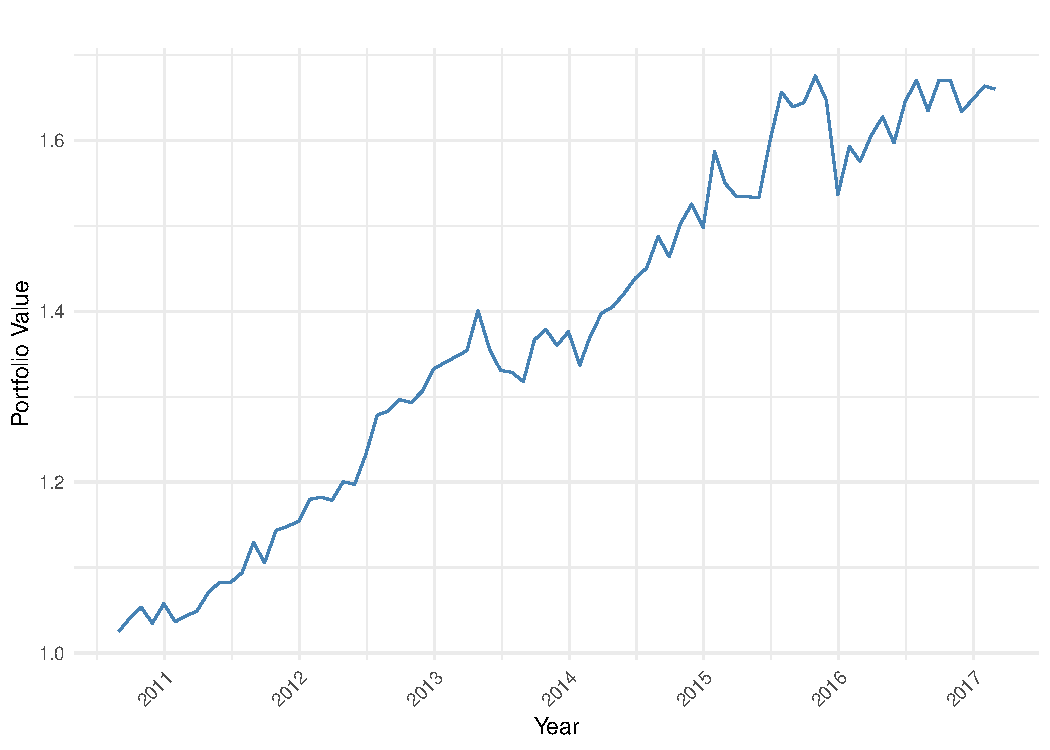
\includegraphics{NDXNES005_A1_RMD_files/figure-latex/unnamed-chunk-9-1.pdf}

\subsubsection{1.10 Final cumulative
return}\label{final-cumulative-return}

\begin{Shaded}
\begin{Highlighting}[]
\NormalTok{final\_ret }\OtherTok{\textless{}{-}} \FunctionTok{tail}\NormalTok{(port\_cum, }\DecValTok{1}\NormalTok{)}
\NormalTok{tang\_ret  }\OtherTok{\textless{}{-}} \FunctionTok{prod}\NormalTok{(}\DecValTok{1} \SpecialCharTok{+}\NormalTok{ tst.rets }\SpecialCharTok{\%*\%}\NormalTok{ w\_hat) }\SpecialCharTok{{-}} \DecValTok{1}
\NormalTok{BH\_summary }\OtherTok{\textless{}{-}} \FunctionTok{data.frame}\NormalTok{(}
  \AttributeTok{Window =} \DecValTok{1}\NormalTok{,}
  \AttributeTok{BH\_Return =}\NormalTok{ final\_ret,}
  \AttributeTok{Tangency\_Expected =}\NormalTok{ tang\_ret}
\NormalTok{)}
\NormalTok{knitr}\SpecialCharTok{::}\FunctionTok{kable}\NormalTok{(BH\_summary, }\AttributeTok{digits=}\DecValTok{4}\NormalTok{, }\AttributeTok{caption=}\StringTok{"Buy{-}and{-}Hold Cumulative Return vs Tangency Expected Return"}\NormalTok{)}
\end{Highlighting}
\end{Shaded}

\begin{longtable}[]{@{}rrr@{}}
\caption{Buy-and-Hold Cumulative Return vs Tangency Expected
Return}\tabularnewline
\toprule\noalign{}
Window & BH\_Return & Tangency\_Expected \\
\midrule\noalign{}
\endfirsthead
\toprule\noalign{}
Window & BH\_Return & Tangency\_Expected \\
\midrule\noalign{}
\endhead
\bottomrule\noalign{}
\endlastfoot
1 & 1.6601 & 0.6601 \\
\end{longtable}

\subsection{Experiment 2 : Out-Of-Sample Backtesting using a Rolling
Window}\label{experiment-2-out-of-sample-backtesting-using-a-rolling-window}

\subsubsection{2.1 Libraries (Gebbie,
2025d)}\label{libraries-tim_prep-1}

\begin{Shaded}
\begin{Highlighting}[]
\CommentTok{\# load required libraries}
\FunctionTok{suppressPackageStartupMessages}\NormalTok{(\{}
\FunctionTok{library}\NormalTok{(openxlsx)     }
\FunctionTok{library}\NormalTok{(timeSeries)   }
\FunctionTok{library}\NormalTok{(xts)          }
\FunctionTok{library}\NormalTok{(zoo)          }
\FunctionTok{library}\NormalTok{(matrixStats) }
\FunctionTok{library}\NormalTok{(quadprog)     }
\FunctionTok{library}\NormalTok{(knitr)        }
\FunctionTok{library}\NormalTok{(dplyr)        }
\FunctionTok{library}\NormalTok{(ggplot2)      }
\FunctionTok{library}\NormalTok{(tidyr)  }
\NormalTok{\})}
\end{Highlighting}
\end{Shaded}

\subsubsection{2.2 Load data and preprocessing (Gebbie,
2025d)}\label{load-data-and-preprocessing-tim_prep-1}

\begin{Shaded}
\begin{Highlighting}[]
\CommentTok{\# reading in all 4 sheets into a list}
\NormalTok{dfS }\OtherTok{\textless{}{-}} \FunctionTok{list}\NormalTok{()}
\ControlFlowTok{for}\NormalTok{ (i }\ControlFlowTok{in} \DecValTok{1}\SpecialCharTok{:}\DecValTok{4}\NormalTok{) \{}
\NormalTok{  dfS[[i]] }\OtherTok{\textless{}{-}} \FunctionTok{read.xlsx}\NormalTok{(}\StringTok{"\_raw\_data/PT{-}TAA{-}JSE{-}Daily{-}1994{-}2017.xlsx"}\NormalTok{, }\AttributeTok{sheet =}\NormalTok{ i, }\AttributeTok{detectDates =} \ConstantTok{TRUE}\NormalTok{)}
  \FunctionTok{cat}\NormalTok{(}\StringTok{"Sheet"}\NormalTok{, i, }\StringTok{"loaded with dimensions:"}\NormalTok{, }\FunctionTok{dim}\NormalTok{(dfS[[i]]), }\StringTok{"}\SpecialCharTok{\textbackslash{}n}\StringTok{"}\NormalTok{)}
\NormalTok{\}}
\end{Highlighting}
\end{Shaded}

\begin{verbatim}
## Sheet 1 loaded with dimensions: 8439 2 
## Sheet 2 loaded with dimensions: 8405 4 
## Sheet 3 loaded with dimensions: 8439 28 
## Sheet 4 loaded with dimensions: 8439 20
\end{verbatim}

\begin{Shaded}
\begin{Highlighting}[]
\CommentTok{\# define entities and which assets to keep}
\NormalTok{Entities }\OtherTok{\textless{}{-}} \FunctionTok{c}\NormalTok{(}\StringTok{\textquotesingle{}X1\textquotesingle{}}\NormalTok{,}\StringTok{\textquotesingle{}STEFI\textquotesingle{}}\NormalTok{,}\StringTok{\textquotesingle{}ALBI\textquotesingle{}}\NormalTok{,}\StringTok{\textquotesingle{}J203\textquotesingle{}}\NormalTok{,}\StringTok{\textquotesingle{}J500\textquotesingle{}}\NormalTok{, }\FunctionTok{sprintf}\NormalTok{(}\StringTok{"J5\%d"}\NormalTok{, }\FunctionTok{seq}\NormalTok{(}\DecValTok{10}\NormalTok{,}\DecValTok{90}\NormalTok{,}\AttributeTok{by=}\DecValTok{10}\NormalTok{)))}
\NormalTok{Items    }\OtherTok{\textless{}{-}} \FunctionTok{c}\NormalTok{(}\StringTok{\textquotesingle{}Date\textquotesingle{}}\NormalTok{,}\StringTok{\textquotesingle{}TRI\textquotesingle{}}\NormalTok{,}\StringTok{\textquotesingle{}Stefi\textquotesingle{}}\NormalTok{)}

\CommentTok{\#cleaning each sheet}
\ControlFlowTok{for}\NormalTok{ (i }\ControlFlowTok{in} \DecValTok{1}\SpecialCharTok{:}\DecValTok{4}\NormalTok{) \{}
\NormalTok{  tI0 }\OtherTok{\textless{}{-}} \FunctionTok{sapply}\NormalTok{(}\FunctionTok{colnames}\NormalTok{(dfS[[i]]), }\ControlFlowTok{function}\NormalTok{(x) }\FunctionTok{any}\NormalTok{(}\FunctionTok{grepl}\NormalTok{(}\FunctionTok{paste}\NormalTok{(Entities, }\AttributeTok{collapse=}\StringTok{"|"}\NormalTok{), x)))}
\NormalTok{  tI1 }\OtherTok{\textless{}{-}} \FunctionTok{sapply}\NormalTok{(dfS[[i]][}\DecValTok{2}\NormalTok{,], }\ControlFlowTok{function}\NormalTok{(x) }\FunctionTok{any}\NormalTok{(}\FunctionTok{grepl}\NormalTok{(}\FunctionTok{paste}\NormalTok{(Items, }\AttributeTok{collapse=}\StringTok{"|"}\NormalTok{), x)))}
\NormalTok{  tI  }\OtherTok{\textless{}{-}}\NormalTok{ tI0 }\SpecialCharTok{\&}\NormalTok{ tI1}
  
  \CommentTok{\# remove header rows}
\NormalTok{  dfS[[i]] }\OtherTok{\textless{}{-}}\NormalTok{ dfS[[i]][}\SpecialCharTok{{-}}\FunctionTok{c}\NormalTok{(}\DecValTok{1}\NormalTok{,}\DecValTok{2}\NormalTok{), tI]}
  \FunctionTok{names}\NormalTok{(dfS[[i]])[}\DecValTok{1}\NormalTok{] }\OtherTok{\textless{}{-}} \StringTok{"Date"}
  
\NormalTok{  newColNames }\OtherTok{\textless{}{-}} \FunctionTok{strsplit}\NormalTok{(}\FunctionTok{colnames}\NormalTok{(dfS[[i]]), }\StringTok{":"}\NormalTok{)}
  \ControlFlowTok{for}\NormalTok{(m }\ControlFlowTok{in} \DecValTok{2}\SpecialCharTok{:}\FunctionTok{length}\NormalTok{(newColNames)) }\FunctionTok{names}\NormalTok{(dfS[[i]])[m] }\OtherTok{\textless{}{-}}\NormalTok{ newColNames[[m]][}\DecValTok{1}\NormalTok{]}
  
  \FunctionTok{cat}\NormalTok{(}\StringTok{"Sheet"}\NormalTok{, i, }\StringTok{"columns after cleaning:"}\NormalTok{, }\FunctionTok{colnames}\NormalTok{(dfS[[i]]), }\StringTok{"}\SpecialCharTok{\textbackslash{}n}\StringTok{"}\NormalTok{)}
\NormalTok{\}}
\end{Highlighting}
\end{Shaded}

\begin{verbatim}
## Sheet 1 columns after cleaning: Date ALBI 
## Sheet 2 columns after cleaning: Date RATESTEFI 
## Sheet 3 columns after cleaning: Date J500 J510 J520 J530 J540 J550 J560 J580 J590 
## Sheet 4 columns after cleaning: Date J203
\end{verbatim}

\begin{Shaded}
\begin{Highlighting}[]
\CommentTok{\# fixing ALBI column}
\NormalTok{dfS[[}\DecValTok{1}\NormalTok{]][,}\DecValTok{2}\NormalTok{] }\OtherTok{\textless{}{-}} \FunctionTok{as.numeric}\NormalTok{(dfS[[}\DecValTok{1}\NormalTok{]][,}\DecValTok{2}\NormalTok{])  }
\NormalTok{dfS[[}\DecValTok{1}\NormalTok{]] }\OtherTok{\textless{}{-}}\NormalTok{ dfS[[}\DecValTok{1}\NormalTok{]][}\SpecialCharTok{!}\FunctionTok{is.na}\NormalTok{(dfS[[}\DecValTok{1}\NormalTok{]][,}\DecValTok{2}\NormalTok{]), ]}\CommentTok{\#removes rows where ALBI is NA}
\end{Highlighting}
\end{Shaded}

\subsubsection{2.3 Merge into single timeSeries object (Gebbie,
2025d)}\label{merge-into-single-timeseries-object-tim_prep-1}

\begin{Shaded}
\begin{Highlighting}[]
\CommentTok{\# converts first sheet to timeSeries}
\NormalTok{tsTAA }\OtherTok{\textless{}{-}} \FunctionTok{timeSeries}\NormalTok{(dfS[[}\DecValTok{1}\NormalTok{]][, }\DecValTok{2}\SpecialCharTok{:}\FunctionTok{ncol}\NormalTok{(dfS[[}\DecValTok{1}\NormalTok{]])], }\FunctionTok{as.Date}\NormalTok{(dfS[[}\DecValTok{1}\NormalTok{]][,}\DecValTok{1}\NormalTok{]))}
\FunctionTok{cat}\NormalTok{(}\StringTok{"Initial tsTAA dimensions:"}\NormalTok{, }\FunctionTok{dim}\NormalTok{(tsTAA), }\StringTok{"}\SpecialCharTok{\textbackslash{}n}\StringTok{"}\NormalTok{)}
\end{Highlighting}
\end{Shaded}

\begin{verbatim}
## Initial tsTAA dimensions: 4324 1
\end{verbatim}

\begin{Shaded}
\begin{Highlighting}[]
\CommentTok{\# merges remaining sheets}
\ControlFlowTok{for}\NormalTok{ (i }\ControlFlowTok{in} \DecValTok{2}\SpecialCharTok{:}\DecValTok{4}\NormalTok{) \{}
\NormalTok{  tsTmp }\OtherTok{\textless{}{-}} \FunctionTok{timeSeries}\NormalTok{(dfS[[i]][, }\DecValTok{2}\SpecialCharTok{:}\FunctionTok{ncol}\NormalTok{(dfS[[i]])], }\FunctionTok{as.Date}\NormalTok{(dfS[[i]][,}\DecValTok{1}\NormalTok{]))}
\NormalTok{  tsTAA }\OtherTok{\textless{}{-}} \FunctionTok{cbind}\NormalTok{(tsTAA, tsTmp)}
  \FunctionTok{cat}\NormalTok{(}\StringTok{"After merging sheet"}\NormalTok{, i, }\StringTok{"dimensions:"}\NormalTok{, }\FunctionTok{dim}\NormalTok{(tsTAA), }\StringTok{"}\SpecialCharTok{\textbackslash{}n}\StringTok{"}\NormalTok{)}
\NormalTok{\}}
\end{Highlighting}
\end{Shaded}

\begin{verbatim}
## After merging sheet 2 dimensions: 8437 2 
## After merging sheet 3 dimensions: 8437 11 
## After merging sheet 4 dimensions: 8437 12
\end{verbatim}

\begin{Shaded}
\begin{Highlighting}[]
\CommentTok{\# renaming indices for clarity}
\FunctionTok{setFinCenter}\NormalTok{(tsTAA) }\OtherTok{\textless{}{-}} \StringTok{"Johannesburg"}
\FunctionTok{names}\NormalTok{(tsTAA)[}\FunctionTok{grep}\NormalTok{(}\StringTok{"TS.1.1"}\NormalTok{, }\FunctionTok{names}\NormalTok{(tsTAA))] }\OtherTok{\textless{}{-}} \StringTok{"ALBI"}
\FunctionTok{names}\NormalTok{(tsTAA)[}\FunctionTok{grep}\NormalTok{(}\StringTok{"TS.1.2"}\NormalTok{, }\FunctionTok{names}\NormalTok{(tsTAA))] }\OtherTok{\textless{}{-}} \StringTok{"STEFI"}
\FunctionTok{names}\NormalTok{(tsTAA)[}\FunctionTok{grep}\NormalTok{(}\StringTok{"TS.1"}\NormalTok{, }\FunctionTok{names}\NormalTok{(tsTAA))] }\OtherTok{\textless{}{-}} \StringTok{"ALSI"}

\FunctionTok{cat}\NormalTok{(}\StringTok{"Columns after renaming:"}\NormalTok{, }\FunctionTok{colnames}\NormalTok{(tsTAA), }\StringTok{"}\SpecialCharTok{\textbackslash{}n}\StringTok{"}\NormalTok{)}
\end{Highlighting}
\end{Shaded}

\begin{verbatim}
## Columns after renaming: ALBI STEFI J500 J510 J520 J530 J540 J550 J560 J580 J590 ALSI
\end{verbatim}

\begin{Shaded}
\begin{Highlighting}[]
\CommentTok{\#all numeric columns are numeric}
\ControlFlowTok{for}\NormalTok{ (j }\ControlFlowTok{in} \DecValTok{1}\SpecialCharTok{:}\FunctionTok{ncol}\NormalTok{(tsTAA)) \{}
\NormalTok{  tsTAA[, j] }\OtherTok{\textless{}{-}} \FunctionTok{as.numeric}\NormalTok{(tsTAA[, j])}
\NormalTok{\}}
\CommentTok{\#remove rows with all NAs}
\NormalTok{tsTAA }\OtherTok{\textless{}{-}}\NormalTok{ tsTAA[}\FunctionTok{rowSums}\NormalTok{(}\FunctionTok{is.na}\NormalTok{(tsTAA)) }\SpecialCharTok{\textless{}} \FunctionTok{ncol}\NormalTok{(tsTAA), ]}

\CommentTok{\# Using timeSeries daily2monthly and ensure tsTAA is valid}
\NormalTok{tsTAA\_monthly }\OtherTok{\textless{}{-}} \FunctionTok{tryCatch}\NormalTok{(}
  \FunctionTok{daily2monthly}\NormalTok{(tsTAA),}
  \AttributeTok{error =} \ControlFlowTok{function}\NormalTok{(e) \{}
    \FunctionTok{stop}\NormalTok{(}\StringTok{"Error in daily2monthly: tsTAA might contain non{-}timeSeries columns or non{-}numeric values"}\NormalTok{)}
\NormalTok{  \}}
\NormalTok{)}

\CommentTok{\#  monthly price index}
\NormalTok{tsIdx  }\OtherTok{\textless{}{-}} \FunctionTok{index2wealth}\NormalTok{(tsTAA\_monthly)}

\CommentTok{\# geometric monthly returns}
\NormalTok{tsGRet }\OtherTok{\textless{}{-}} \FunctionTok{diff}\NormalTok{(}\FunctionTok{log}\NormalTok{(tsIdx))}

\FunctionTok{cat}\NormalTok{(}\StringTok{"tsTAA\_monthly dimensions:"}\NormalTok{, }\FunctionTok{dim}\NormalTok{(tsTAA\_monthly), }\StringTok{"}\SpecialCharTok{\textbackslash{}n}\StringTok{"}\NormalTok{)}
\end{Highlighting}
\end{Shaded}

\begin{verbatim}
## tsTAA_monthly dimensions: 261 12
\end{verbatim}

\begin{Shaded}
\begin{Highlighting}[]
\FunctionTok{cat}\NormalTok{(}\StringTok{"tsGRet dimensions:"}\NormalTok{, }\FunctionTok{dim}\NormalTok{(tsGRet), }\StringTok{"}\SpecialCharTok{\textbackslash{}n}\StringTok{"}\NormalTok{)}
\end{Highlighting}
\end{Shaded}

\begin{verbatim}
## tsGRet dimensions: 261 12
\end{verbatim}

\begin{Shaded}
\begin{Highlighting}[]
\FunctionTok{cat}\NormalTok{(}\StringTok{"Columns in tsGRet:}\SpecialCharTok{\textbackslash{}n}\StringTok{"}\NormalTok{); }\FunctionTok{print}\NormalTok{(}\FunctionTok{colnames}\NormalTok{(tsGRet))}
\end{Highlighting}
\end{Shaded}

\begin{verbatim}
## Columns in tsGRet:
\end{verbatim}

\begin{verbatim}
##  [1] "ALBI"  "STEFI" "J500"  "J510"  "J520"  "J530"  "J540"  "J550"  "J560" 
## [10] "J580"  "J590"  "ALSI"
\end{verbatim}

\subsubsection{2.4 Arithmetic Returns (Gebbie,
2025c)}\label{arithmetic-returns-tim_btmlx-1}

\begin{Shaded}
\begin{Highlighting}[]
\FunctionTok{setFinCenter}\NormalTok{(tsTAA) }\OtherTok{\textless{}{-}} \StringTok{"Africa/Johannesburg"}
\FunctionTok{summary}\NormalTok{(dfS[[}\DecValTok{1}\NormalTok{]][,}\DecValTok{2}\NormalTok{])}
\end{Highlighting}
\end{Shaded}

\begin{verbatim}
##    Min. 1st Qu.  Median    Mean 3rd Qu.    Max. 
##   173.7   256.9   343.9   357.5   442.0   545.9
\end{verbatim}

\begin{Shaded}
\begin{Highlighting}[]
\CommentTok{\# Checks that tsTAA is a proper \textquotesingle{}timeSeries\textquotesingle{} object}
\NormalTok{tsTAA\_monthly }\OtherTok{\textless{}{-}} \FunctionTok{tryCatch}\NormalTok{(}
  \FunctionTok{daily2monthly}\NormalTok{(tsTAA),}
  \AttributeTok{error =} \ControlFlowTok{function}\NormalTok{(e) \{}
    \FunctionTok{message}\NormalTok{(}\StringTok{"Error in daily2monthly(): converting tsTAA to xts first"}\NormalTok{)}
\NormalTok{    xts\_obj }\OtherTok{\textless{}{-}} \FunctionTok{as.xts}\NormalTok{(tsTAA)}
    \FunctionTok{apply.monthly}\NormalTok{(xts\_obj, colMeans, }\AttributeTok{na.rm=}\ConstantTok{TRUE}\NormalTok{)}
\NormalTok{  \}}
\NormalTok{)}



\CommentTok{\#geometric returns}
\NormalTok{tsGRet }\OtherTok{\textless{}{-}} \FunctionTok{diff}\NormalTok{(}\FunctionTok{log}\NormalTok{(tsTAA\_monthly))}

\CommentTok{\#  fill missing data using LOCF}
\NormalTok{tsGRet\_filled }\OtherTok{\textless{}{-}} \FunctionTok{na.locf}\NormalTok{(}\FunctionTok{as.xts}\NormalTok{(tsGRet), }\AttributeTok{na.rm =} \ConstantTok{FALSE}\NormalTok{)}
\FunctionTok{summary}\NormalTok{(tsGRet\_filled[,}\StringTok{"ALBI"}\NormalTok{])}
\end{Highlighting}
\end{Shaded}

\begin{verbatim}
##      Index                             ALBI         
##  Min.   :1995-06-30 00:00:00.00   Min.   :-0.06908  
##  1st Qu.:2000-11-30 00:00:00.00   1st Qu.:-0.00232  
##  Median :2006-04-30 00:00:00.00   Median : 0.00362  
##  Mean   :2006-04-30 22:31:43.45   Mean   : 0.00701  
##  3rd Qu.:2011-09-30 00:00:00.00   3rd Qu.: 0.01581  
##  Max.   :2017-02-28 00:00:00.00   Max.   : 0.16900  
##                                   NA's   :99
\end{verbatim}

\begin{Shaded}
\begin{Highlighting}[]
\FunctionTok{any}\NormalTok{(}\SpecialCharTok{!}\FunctionTok{is.na}\NormalTok{(tsGRet\_filled[,}\StringTok{"ALBI"}\NormalTok{]))}
\end{Highlighting}
\end{Shaded}

\begin{verbatim}
## [1] TRUE
\end{verbatim}

\begin{Shaded}
\begin{Highlighting}[]
\CommentTok{\#checking for columns that are all NA}
\NormalTok{cols\_allNA }\OtherTok{\textless{}{-}} \FunctionTok{colSums}\NormalTok{(}\SpecialCharTok{!}\FunctionTok{is.na}\NormalTok{(tsGRet\_filled)) }\SpecialCharTok{==} \DecValTok{0}
\NormalTok{tsGRet\_filled }\OtherTok{\textless{}{-}}\NormalTok{ tsGRet\_filled[, }\SpecialCharTok{!}\NormalTok{cols\_allNA]}

\CommentTok{\# converting to arithmetic returns}
\NormalTok{simple\_mat }\OtherTok{\textless{}{-}} \FunctionTok{exp}\NormalTok{(}\FunctionTok{as.matrix}\NormalTok{(tsGRet\_filled)) }\SpecialCharTok{{-}} \DecValTok{1}
\NormalTok{rets\_xts }\OtherTok{\textless{}{-}} \FunctionTok{xts}\NormalTok{(simple\_mat, }\AttributeTok{order.by =} \FunctionTok{index}\NormalTok{(tsGRet\_filled))}
\FunctionTok{colnames}\NormalTok{(rets\_xts) }\OtherTok{\textless{}{-}} \FunctionTok{colnames}\NormalTok{(tsGRet\_filled)}

\CommentTok{\# Excludes cash asset}
\NormalTok{cash\_idx }\OtherTok{\textless{}{-}} \FunctionTok{grep}\NormalTok{(}\StringTok{"STEFI"}\NormalTok{, }\FunctionTok{colnames}\NormalTok{(rets\_xts), }\AttributeTok{ignore.case =} \ConstantTok{TRUE}\NormalTok{)}
\NormalTok{cash\_name }\OtherTok{\textless{}{-}} \FunctionTok{ifelse}\NormalTok{(}\FunctionTok{length}\NormalTok{(cash\_idx) }\SpecialCharTok{\textgreater{}} \DecValTok{0}\NormalTok{, }\FunctionTok{colnames}\NormalTok{(rets\_xts)[cash\_idx[}\DecValTok{1}\NormalTok{]], }\ConstantTok{NA}\NormalTok{)}

\NormalTok{rets\_opt }\OtherTok{\textless{}{-}} \ControlFlowTok{if}\NormalTok{(}\SpecialCharTok{!}\FunctionTok{is.na}\NormalTok{(cash\_name)) rets\_xts[, }\SpecialCharTok{{-}}\NormalTok{cash\_idx, drop}\OtherTok{=}\ConstantTok{FALSE}\NormalTok{] }\ControlFlowTok{else}\NormalTok{ rets\_xts}
\NormalTok{rets\_cash }\OtherTok{\textless{}{-}} \ControlFlowTok{if}\NormalTok{(}\SpecialCharTok{!}\FunctionTok{is.na}\NormalTok{(cash\_name)) rets\_xts[, cash\_idx, drop}\OtherTok{=}\ConstantTok{FALSE}\NormalTok{] }\ControlFlowTok{else} \ConstantTok{NULL}

\FunctionTok{cat}\NormalTok{(}\StringTok{"Assets used for optimisation:}\SpecialCharTok{\textbackslash{}n}\StringTok{"}\NormalTok{); }\FunctionTok{print}\NormalTok{(}\FunctionTok{colnames}\NormalTok{(rets\_opt))}
\end{Highlighting}
\end{Shaded}

\begin{verbatim}
## Assets used for optimisation:
\end{verbatim}

\begin{verbatim}
##  [1] "ALBI" "J500" "J510" "J520" "J530" "J540" "J550" "J560" "J580" "J590"
## [11] "ALSI"
\end{verbatim}

\begin{Shaded}
\begin{Highlighting}[]
\ControlFlowTok{if}\NormalTok{(}\SpecialCharTok{!}\FunctionTok{is.na}\NormalTok{(cash\_name)) }\FunctionTok{cat}\NormalTok{(}\StringTok{"Cash excluded from optimisation:"}\NormalTok{, cash\_name, }\StringTok{"}\SpecialCharTok{\textbackslash{}n}\StringTok{"}\NormalTok{)}
\end{Highlighting}
\end{Shaded}

\begin{verbatim}
## Cash excluded from optimisation: STEFI
\end{verbatim}

\subsubsection{2.5 Tangency Portfolio (Gebbie, 2025c,
2025d)}\label{tangency-portfolio-tim_btmlx-tim_prep}

\begin{Shaded}
\begin{Highlighting}[]
\NormalTok{tan.port }\OtherTok{\textless{}{-}} \ControlFlowTok{function}\NormalTok{(mu, Sigma, }\AttributeTok{rf=}\DecValTok{0}\NormalTok{, }\AttributeTok{targets=}\FunctionTok{seq}\NormalTok{(}\FloatTok{0.001}\NormalTok{,}\FloatTok{0.05}\NormalTok{,}\AttributeTok{length.out=}\DecValTok{200}\NormalTok{))\{}
\NormalTok{  n }\OtherTok{\textless{}{-}} \FunctionTok{length}\NormalTok{(mu)}
\NormalTok{  Dmat }\OtherTok{\textless{}{-}} \DecValTok{2}\SpecialCharTok{*}\NormalTok{(Sigma }\SpecialCharTok{+} \FunctionTok{diag}\NormalTok{(}\FloatTok{1e{-}8}\NormalTok{,n))  }\CommentTok{\# ensure PD covariance}
\NormalTok{  best }\OtherTok{\textless{}{-}} \FunctionTok{list}\NormalTok{(}\AttributeTok{sharpe=}\SpecialCharTok{{-}}\ConstantTok{Inf}\NormalTok{)}
  
  \ControlFlowTok{for}\NormalTok{(tgt }\ControlFlowTok{in}\NormalTok{ targets)\{}
\NormalTok{    gamma }\OtherTok{\textless{}{-}} \FunctionTok{as.numeric}\NormalTok{(mu }\SpecialCharTok{{-}}\NormalTok{ rf)}
\NormalTok{    Amat }\OtherTok{\textless{}{-}} \FunctionTok{cbind}\NormalTok{(gamma, }\SpecialCharTok{{-}}\NormalTok{gamma, }\FunctionTok{rep}\NormalTok{(}\DecValTok{1}\NormalTok{,n), }\SpecialCharTok{{-}}\FunctionTok{rep}\NormalTok{(}\DecValTok{1}\NormalTok{,n), }\FunctionTok{diag}\NormalTok{(n))}
\NormalTok{    bvec }\OtherTok{\textless{}{-}} \FunctionTok{c}\NormalTok{(tgt, }\SpecialCharTok{{-}}\NormalTok{tgt, }\DecValTok{1}\NormalTok{, }\SpecialCharTok{{-}}\DecValTok{1}\NormalTok{, }\FunctionTok{rep}\NormalTok{(}\DecValTok{0}\NormalTok{,n))}
\NormalTok{    sol }\OtherTok{\textless{}{-}} \FunctionTok{try}\NormalTok{(}\FunctionTok{solve.QP}\NormalTok{(Dmat, }\AttributeTok{dvec=}\FunctionTok{rep}\NormalTok{(}\DecValTok{0}\NormalTok{,n), }\AttributeTok{Amat=}\FunctionTok{as.matrix}\NormalTok{(Amat), }\AttributeTok{bvec=}\NormalTok{bvec, }\AttributeTok{meq=}\DecValTok{0}\NormalTok{), }\AttributeTok{silent=}\ConstantTok{TRUE}\NormalTok{)}
    \ControlFlowTok{if}\NormalTok{(}\FunctionTok{inherits}\NormalTok{(sol,}\StringTok{"try{-}error"}\NormalTok{)) }\ControlFlowTok{next}
\NormalTok{    w }\OtherTok{\textless{}{-}}\NormalTok{ sol}\SpecialCharTok{$}\NormalTok{solution}
\NormalTok{    w[w}\SpecialCharTok{\textless{}}\FloatTok{1e{-}8}\NormalTok{] }\OtherTok{\textless{}{-}} \DecValTok{0}
    \ControlFlowTok{if}\NormalTok{(}\FunctionTok{sum}\NormalTok{(w)}\SpecialCharTok{\textless{}=}\DecValTok{0}\NormalTok{) }\ControlFlowTok{next}
\NormalTok{    w }\OtherTok{\textless{}{-}}\NormalTok{ w}\SpecialCharTok{/}\FunctionTok{sum}\NormalTok{(w)}
\NormalTok{    port\_mean }\OtherTok{\textless{}{-}} \FunctionTok{sum}\NormalTok{(w}\SpecialCharTok{*}\NormalTok{mu)}
\NormalTok{    port\_var  }\OtherTok{\textless{}{-}} \FunctionTok{as.numeric}\NormalTok{(}\FunctionTok{t}\NormalTok{(w) }\SpecialCharTok{\%*\%}\NormalTok{ Sigma }\SpecialCharTok{\%*\%}\NormalTok{ w)}
    \ControlFlowTok{if}\NormalTok{(port\_var}\SpecialCharTok{\textless{}=}\DecValTok{0}\NormalTok{) }\ControlFlowTok{next}
\NormalTok{    sr }\OtherTok{\textless{}{-}}\NormalTok{ (port\_mean }\SpecialCharTok{{-}}\NormalTok{ rf)}\SpecialCharTok{/}\FunctionTok{sqrt}\NormalTok{(port\_var)}
    \ControlFlowTok{if}\NormalTok{(sr }\SpecialCharTok{\textgreater{}}\NormalTok{ best}\SpecialCharTok{$}\NormalTok{sharpe) best }\OtherTok{\textless{}{-}} \FunctionTok{list}\NormalTok{(}\AttributeTok{weights=}\NormalTok{w, }\AttributeTok{target=}\NormalTok{tgt, }\AttributeTok{sharpe=}\NormalTok{sr, }\AttributeTok{mean=}\NormalTok{port\_mean, }\AttributeTok{var=}\NormalTok{port\_var)}
\NormalTok{  \}}
  \FunctionTok{return}\NormalTok{(best)}
\NormalTok{\}}
\end{Highlighting}
\end{Shaded}

\subsubsection{2.6 Rolling Window Experiment (Gebbie, 2025c,
2025d)}\label{rolling-window-experiment-tim_btmlx-tim_prep}

\begin{Shaded}
\begin{Highlighting}[]
\NormalTok{train.m }\OtherTok{\textless{}{-}} \DecValTok{60} \CommentTok{\# 5 year period}
\NormalTok{test.m  }\OtherTok{\textless{}{-}} \DecValTok{12} \CommentTok{\# 1 year period}
\NormalTok{roll\_step }\OtherTok{\textless{}{-}} \DecValTok{1} \CommentTok{\#1 month increments}
\NormalTok{n\_obs }\OtherTok{\textless{}{-}} \FunctionTok{nrow}\NormalTok{(rets\_opt)}
\NormalTok{start\_idxs }\OtherTok{\textless{}{-}} \FunctionTok{seq}\NormalTok{(}\DecValTok{1}\NormalTok{, n\_obs }\SpecialCharTok{{-}}\NormalTok{ train.m }\SpecialCharTok{{-}}\NormalTok{ test.m }\SpecialCharTok{+} \DecValTok{1}\NormalTok{, }\AttributeTok{by=}\NormalTok{roll\_step)}
\NormalTok{results }\OtherTok{\textless{}{-}} \FunctionTok{list}\NormalTok{()}

\ControlFlowTok{for}\NormalTok{(i }\ControlFlowTok{in} \FunctionTok{seq\_along}\NormalTok{(start\_idxs))\{}
\NormalTok{  s }\OtherTok{\textless{}{-}}\NormalTok{ start\_idxs[i]}
\NormalTok{  train\_idx }\OtherTok{\textless{}{-}}\NormalTok{ s}\SpecialCharTok{:}\NormalTok{(s}\SpecialCharTok{+}\NormalTok{train.m}\DecValTok{{-}1}\NormalTok{)}
\NormalTok{  tst.idx  }\OtherTok{\textless{}{-}}\NormalTok{ (s}\SpecialCharTok{+}\NormalTok{train.m)}\SpecialCharTok{:}\NormalTok{(s}\SpecialCharTok{+}\NormalTok{train.m}\SpecialCharTok{+}\NormalTok{test.m}\DecValTok{{-}1}\NormalTok{)}
  
\NormalTok{  train\_rets }\OtherTok{\textless{}{-}}\NormalTok{ rets\_opt[train\_idx, , drop}\OtherTok{=}\ConstantTok{FALSE}\NormalTok{]}
\NormalTok{  tst.rets  }\OtherTok{\textless{}{-}}\NormalTok{ rets\_opt[tst.idx, , drop}\OtherTok{=}\ConstantTok{FALSE}\NormalTok{]}
  
  \ControlFlowTok{if}\NormalTok{(}\FunctionTok{any}\NormalTok{(}\SpecialCharTok{!}\FunctionTok{is.finite}\NormalTok{(}\FunctionTok{as.matrix}\NormalTok{(train\_rets))) }\SpecialCharTok{||} \FunctionTok{any}\NormalTok{(}\SpecialCharTok{!}\FunctionTok{is.finite}\NormalTok{(}\FunctionTok{as.matrix}\NormalTok{(tst.rets)))) }\ControlFlowTok{next}
  
\NormalTok{  mu\_train    }\OtherTok{\textless{}{-}} \FunctionTok{colMeans}\NormalTok{(train\_rets, }\AttributeTok{na.rm=}\ConstantTok{TRUE}\NormalTok{)}
\NormalTok{ Sigma\_train }\OtherTok{\textless{}{-}} \FunctionTok{cov}\NormalTok{(}\FunctionTok{as.matrix}\NormalTok{(train\_rets), }\AttributeTok{use=}\StringTok{"complete.obs"}\NormalTok{)}

\NormalTok{  rf\_train    }\OtherTok{\textless{}{-}} \ControlFlowTok{if}\NormalTok{(}\SpecialCharTok{!}\FunctionTok{is.null}\NormalTok{(rets\_cash)) }\FunctionTok{mean}\NormalTok{(rets\_cash[train\_idx, ], }\AttributeTok{na.rm=}\ConstantTok{TRUE}\NormalTok{) }\ControlFlowTok{else} \DecValTok{0}
\NormalTok{  rf\_test     }\OtherTok{\textless{}{-}} \ControlFlowTok{if}\NormalTok{(}\SpecialCharTok{!}\FunctionTok{is.null}\NormalTok{(rets\_cash)) }\FunctionTok{mean}\NormalTok{(rets\_cash[tst.idx, ], }\AttributeTok{na.rm=}\ConstantTok{TRUE}\NormalTok{) }\ControlFlowTok{else} \DecValTok{0}
  
  \CommentTok{\# Skip invalid windows}
  \ControlFlowTok{if}\NormalTok{(}\FunctionTok{any}\NormalTok{(}\SpecialCharTok{!}\FunctionTok{is.finite}\NormalTok{(mu\_train)) }\SpecialCharTok{||} \SpecialCharTok{!}\FunctionTok{is.finite}\NormalTok{(rf\_train)) }\ControlFlowTok{next}
\NormalTok{  upper\_targ }\OtherTok{\textless{}{-}} \FunctionTok{max}\NormalTok{(}\FloatTok{0.06}\NormalTok{, }\FunctionTok{max}\NormalTok{(mu\_train, }\AttributeTok{na.rm=}\ConstantTok{TRUE}\NormalTok{) }\SpecialCharTok{{-}}\NormalTok{ rf\_train)}
  \ControlFlowTok{if}\NormalTok{(}\SpecialCharTok{!}\FunctionTok{is.finite}\NormalTok{(upper\_targ) }\SpecialCharTok{||}\NormalTok{ upper\_targ }\SpecialCharTok{\textless{}=} \DecValTok{0}\NormalTok{) }\ControlFlowTok{next}
  
\NormalTok{  targ\_grid }\OtherTok{\textless{}{-}} \FunctionTok{seq}\NormalTok{(}\FloatTok{0.0005}\NormalTok{, upper\_targ, }\AttributeTok{length.out=}\DecValTok{300}\NormalTok{)}
\NormalTok{  tang }\OtherTok{\textless{}{-}} \FunctionTok{tan.port}\NormalTok{(}\AttributeTok{mu=}\NormalTok{mu\_train, }\AttributeTok{Sigma=}\NormalTok{Sigma\_train, }\AttributeTok{rf=}\NormalTok{rf\_train, }\AttributeTok{targets=}\NormalTok{targ\_grid)}
  \ControlFlowTok{if}\NormalTok{(}\FunctionTok{is.null}\NormalTok{(tang}\SpecialCharTok{$}\NormalTok{weights)) }\ControlFlowTok{next}
  
\NormalTok{  w\_hat }\OtherTok{\textless{}{-}}\NormalTok{ tang}\SpecialCharTok{$}\NormalTok{weights}
\NormalTok{  port\_train }\OtherTok{\textless{}{-}} \FunctionTok{as.numeric}\NormalTok{(}\FunctionTok{as.matrix}\NormalTok{(train\_rets) }\SpecialCharTok{\%*\%}\NormalTok{ w\_hat)}
\NormalTok{  port\_test  }\OtherTok{\textless{}{-}} \FunctionTok{as.numeric}\NormalTok{(}\FunctionTok{as.matrix}\NormalTok{(tst.rets) }\SpecialCharTok{\%*\%}\NormalTok{ w\_hat)}

  
\NormalTok{  results[[}\FunctionTok{length}\NormalTok{(results)}\SpecialCharTok{+}\DecValTok{1}\NormalTok{]] }\OtherTok{\textless{}{-}} \FunctionTok{list}\NormalTok{(}
    \AttributeTok{train\_period =} \FunctionTok{paste}\NormalTok{(}\FunctionTok{index}\NormalTok{(train\_rets)[}\DecValTok{1}\NormalTok{], }\FunctionTok{index}\NormalTok{(train\_rets)[}\FunctionTok{nrow}\NormalTok{(train\_rets)], }\AttributeTok{sep=}\StringTok{" / "}\NormalTok{),}
    \AttributeTok{tst.period  =} \FunctionTok{paste}\NormalTok{(}\FunctionTok{index}\NormalTok{(tst.rets)[}\DecValTok{1}\NormalTok{], }\FunctionTok{index}\NormalTok{(tst.rets)[}\FunctionTok{nrow}\NormalTok{(tst.rets)], }\AttributeTok{sep=}\StringTok{" / "}\NormalTok{),}
    \AttributeTok{mu\_IS =} \FunctionTok{mean}\NormalTok{(port\_train, }\AttributeTok{na.rm=}\ConstantTok{TRUE}\NormalTok{),}
    \AttributeTok{var\_IS=} \FunctionTok{var}\NormalTok{(port\_train, }\AttributeTok{na.rm=}\ConstantTok{TRUE}\NormalTok{),}
    \AttributeTok{SR\_IS =}\NormalTok{(}\FunctionTok{mean}\NormalTok{(port\_train, }\AttributeTok{na.rm=}\ConstantTok{TRUE}\NormalTok{)}\SpecialCharTok{{-}}\NormalTok{rf\_train)}\SpecialCharTok{/}\FunctionTok{sqrt}\NormalTok{(}\FunctionTok{var}\NormalTok{(port\_train, }\AttributeTok{na.rm=}\ConstantTok{TRUE}\NormalTok{)),}
    \AttributeTok{mu\_OOS=} \FunctionTok{mean}\NormalTok{(port\_test, }\AttributeTok{na.rm=}\ConstantTok{TRUE}\NormalTok{),}
    \AttributeTok{var\_OOS=}\FunctionTok{var}\NormalTok{(port\_test, }\AttributeTok{na.rm=}\ConstantTok{TRUE}\NormalTok{),}
    \AttributeTok{SR\_OOS=}\NormalTok{(}\FunctionTok{mean}\NormalTok{(port\_test, }\AttributeTok{na.rm=}\ConstantTok{TRUE}\NormalTok{)}\SpecialCharTok{{-}}\NormalTok{rf\_test)}\SpecialCharTok{/}\FunctionTok{sqrt}\NormalTok{(}\FunctionTok{var}\NormalTok{(port\_test, }\AttributeTok{na.rm=}\ConstantTok{TRUE}\NormalTok{)),}
    \AttributeTok{weights =}\NormalTok{ w\_hat,}
    \AttributeTok{assets  =} \FunctionTok{colnames}\NormalTok{(rets\_opt)}
\NormalTok{  )}
\NormalTok{\}}

\NormalTok{summary\_df }\OtherTok{\textless{}{-}} \FunctionTok{do.call}\NormalTok{(rbind, }\FunctionTok{lapply}\NormalTok{(results, }\ControlFlowTok{function}\NormalTok{(x) }\FunctionTok{data.frame}\NormalTok{(}
  \AttributeTok{train=}\NormalTok{x}\SpecialCharTok{$}\NormalTok{train\_period, }\AttributeTok{test=}\NormalTok{x}\SpecialCharTok{$}\NormalTok{tst.period,}
  \AttributeTok{mu\_IS=}\NormalTok{x}\SpecialCharTok{$}\NormalTok{mu\_IS, }\AttributeTok{var\_IS=}\NormalTok{x}\SpecialCharTok{$}\NormalTok{var\_IS, }\AttributeTok{SR\_IS=}\NormalTok{x}\SpecialCharTok{$}\NormalTok{SR\_IS,}
  \AttributeTok{mu\_OOS=}\NormalTok{x}\SpecialCharTok{$}\NormalTok{mu\_OOS, }\AttributeTok{var\_OOS=}\NormalTok{x}\SpecialCharTok{$}\NormalTok{var\_OOS, }\AttributeTok{SR\_OOS=}\NormalTok{x}\SpecialCharTok{$}\NormalTok{SR\_OOS}
\NormalTok{)))}
\NormalTok{knitr}\SpecialCharTok{::}\FunctionTok{kable}\NormalTok{(}
  \FunctionTok{head}\NormalTok{(summary\_df, }\DecValTok{15}\NormalTok{),}
  \AttributeTok{digits =} \DecValTok{4}\NormalTok{,}
  \AttributeTok{caption =} \StringTok{"In{-}sample vs Out{-}of{-}sample Portfolio Statistics"}
\NormalTok{)}
\end{Highlighting}
\end{Shaded}

\begin{longtable}[]{@{}
  >{\raggedright\arraybackslash}p{(\columnwidth - 14\tabcolsep) * \real{0.2609}}
  >{\raggedright\arraybackslash}p{(\columnwidth - 14\tabcolsep) * \real{0.2609}}
  >{\raggedleft\arraybackslash}p{(\columnwidth - 14\tabcolsep) * \real{0.0761}}
  >{\raggedleft\arraybackslash}p{(\columnwidth - 14\tabcolsep) * \real{0.0761}}
  >{\raggedleft\arraybackslash}p{(\columnwidth - 14\tabcolsep) * \real{0.0761}}
  >{\raggedleft\arraybackslash}p{(\columnwidth - 14\tabcolsep) * \real{0.0761}}
  >{\raggedleft\arraybackslash}p{(\columnwidth - 14\tabcolsep) * \real{0.0870}}
  >{\raggedleft\arraybackslash}p{(\columnwidth - 14\tabcolsep) * \real{0.0870}}@{}}
\caption{In-sample vs Out-of-sample Portfolio Statistics}\tabularnewline
\toprule\noalign{}
\begin{minipage}[b]{\linewidth}\raggedright
train
\end{minipage} & \begin{minipage}[b]{\linewidth}\raggedright
test
\end{minipage} & \begin{minipage}[b]{\linewidth}\raggedleft
mu\_IS
\end{minipage} & \begin{minipage}[b]{\linewidth}\raggedleft
var\_IS
\end{minipage} & \begin{minipage}[b]{\linewidth}\raggedleft
SR\_IS
\end{minipage} & \begin{minipage}[b]{\linewidth}\raggedleft
mu\_OOS
\end{minipage} & \begin{minipage}[b]{\linewidth}\raggedleft
var\_OOS
\end{minipage} & \begin{minipage}[b]{\linewidth}\raggedleft
SR\_OOS
\end{minipage} \\
\midrule\noalign{}
\endfirsthead
\toprule\noalign{}
\begin{minipage}[b]{\linewidth}\raggedright
train
\end{minipage} & \begin{minipage}[b]{\linewidth}\raggedright
test
\end{minipage} & \begin{minipage}[b]{\linewidth}\raggedleft
mu\_IS
\end{minipage} & \begin{minipage}[b]{\linewidth}\raggedleft
var\_IS
\end{minipage} & \begin{minipage}[b]{\linewidth}\raggedleft
SR\_IS
\end{minipage} & \begin{minipage}[b]{\linewidth}\raggedleft
mu\_OOS
\end{minipage} & \begin{minipage}[b]{\linewidth}\raggedleft
var\_OOS
\end{minipage} & \begin{minipage}[b]{\linewidth}\raggedleft
SR\_OOS
\end{minipage} \\
\midrule\noalign{}
\endhead
\bottomrule\noalign{}
\endlastfoot
2003-09-30 / 2008-08-31 & 2008-09-30 / 2009-08-31 & 0.0263 & 0.0020 &
0.4373 & 0.0047 & 0.0063 & -0.0473 \\
2003-10-31 / 2008-09-30 & 2008-10-31 / 2009-09-30 & 0.0253 & 0.0025 &
0.3671 & 0.0095 & 0.0046 & 0.0195 \\
2003-11-30 / 2008-10-31 & 2008-11-30 / 2009-10-31 & 0.0224 & 0.0023 &
0.3205 & 0.0203 & 0.0041 & 0.1956 \\
2003-12-31 / 2008-11-30 & 2008-12-31 / 2009-11-30 & 0.0210 & 0.0022 &
0.2992 & 0.0238 & 0.0043 & 0.2486 \\
2004-01-31 / 2008-12-31 & 2009-01-31 / 2009-12-31 & 0.0196 & 0.0018 &
0.2992 & 0.0195 & 0.0034 & 0.2093 \\
2004-02-29 / 2009-01-31 & 2009-02-28 / 2010-01-31 & 0.0185 & 0.0021 &
0.2492 & 0.0249 & 0.0032 & 0.3206 \\
2004-03-31 / 2009-02-28 & 2009-03-31 / 2010-02-28 & 0.0173 & 0.0024 &
0.2093 & 0.0326 & 0.0017 & 0.6269 \\
2004-04-30 / 2009-03-31 & 2009-04-30 / 2010-03-31 & 0.0180 & 0.0024 &
0.2216 & 0.0291 & 0.0016 & 0.5750 \\
2004-05-31 / 2009-04-30 & 2009-05-31 / 2010-04-30 & 0.0199 & 0.0028 &
0.2431 & 0.0212 & 0.0013 & 0.4085 \\
2004-06-30 / 2009-05-31 & 2009-06-30 / 2010-05-31 & 0.0200 & 0.0024 &
0.2597 & 0.0167 & 0.0017 & 0.2565 \\
2004-07-31 / 2009-06-30 & 2009-07-31 / 2010-06-30 & 0.0208 & 0.0025 &
0.2735 & 0.0143 & 0.0017 & 0.2026 \\
2004-08-31 / 2009-07-31 & 2009-08-31 / 2010-07-31 & 0.0228 & 0.0026 &
0.3068 & 0.0129 & 0.0014 & 0.1862 \\
2004-09-30 / 2009-08-31 & 2009-09-30 / 2010-08-31 & 0.0220 & 0.0025 &
0.2939 & 0.0121 & 0.0014 & 0.1669 \\
2004-10-31 / 2009-09-30 & 2009-10-31 / 2010-09-30 & 0.0212 & 0.0025 &
0.2787 & 0.0204 & 0.0018 & 0.3413 \\
2004-11-30 / 2009-10-31 & 2009-11-30 / 2010-10-31 & 0.0212 & 0.0024 &
0.2864 & 0.0177 & 0.0018 & 0.2836 \\
\end{longtable}

\subsubsection{Plotting In Sample vs Out Of Sample
Statistics}\label{plotting-in-sample-vs-out-of-sample-statistics}

\begin{Shaded}
\begin{Highlighting}[]
\NormalTok{p.dates }\OtherTok{\textless{}{-}} \FunctionTok{as.Date}\NormalTok{(}\FunctionTok{sapply}\NormalTok{(summary\_df}\SpecialCharTok{$}\NormalTok{test, }\ControlFlowTok{function}\NormalTok{(x) \{}
  \FunctionTok{tail}\NormalTok{(}\FunctionTok{strsplit}\NormalTok{(x, }\StringTok{" / "}\NormalTok{)[[}\DecValTok{1}\NormalTok{]], }\DecValTok{1}\NormalTok{)}
\NormalTok{\}), }\AttributeTok{format =} \StringTok{"\%Y{-}\%m{-}\%d"}\NormalTok{)}
\NormalTok{summary\_df}\SpecialCharTok{$}\NormalTok{Date }\OtherTok{\textless{}{-}}\NormalTok{ p.dates  }

\NormalTok{p.long }\OtherTok{\textless{}{-}}\NormalTok{ summary\_df }\SpecialCharTok{|\textgreater{}}
  \FunctionTok{select}\NormalTok{(Date, mu\_IS, var\_IS, SR\_IS, mu\_OOS, var\_OOS, SR\_OOS) }\SpecialCharTok{|\textgreater{}}
  \FunctionTok{pivot\_longer}\NormalTok{(}\SpecialCharTok{{-}}\NormalTok{Date, }\AttributeTok{names\_to =} \StringTok{"Metric"}\NormalTok{, }\AttributeTok{values\_to =} \StringTok{"Value"}\NormalTok{) }\SpecialCharTok{|\textgreater{}}
  \FunctionTok{mutate}\NormalTok{(}
    \AttributeTok{Type   =} \FunctionTok{ifelse}\NormalTok{(}\FunctionTok{grepl}\NormalTok{(}\StringTok{"\_IS"}\NormalTok{, Metric), }\StringTok{"In{-}Sample"}\NormalTok{, }\StringTok{"Out{-}of{-}Sample"}\NormalTok{),}
    \AttributeTok{Metric =} \FunctionTok{gsub}\NormalTok{(}\StringTok{"\_(IS|OOS)"}\NormalTok{, }\StringTok{""}\NormalTok{, Metric)  }
\NormalTok{  ) }\SpecialCharTok{|\textgreater{}}
  \FunctionTok{mutate}\NormalTok{(}
    \AttributeTok{Metric =} \FunctionTok{case\_when}\NormalTok{(}
\NormalTok{      Metric }\SpecialCharTok{==} \StringTok{"mu"}  \SpecialCharTok{\textasciitilde{}} \StringTok{"Mean"}\NormalTok{,}
\NormalTok{      Metric }\SpecialCharTok{==} \StringTok{"var"} \SpecialCharTok{\textasciitilde{}} \StringTok{"Variance"}\NormalTok{,}\ConstantTok{TRUE} \SpecialCharTok{\textasciitilde{}}\NormalTok{ Metric}
\NormalTok{    ))}

\CommentTok{\# Mean and Variance In{-}Sample vs Out{-}of{-}Sample Mean \& Variance}
\NormalTok{p1}\OtherTok{\textless{}{-}}\NormalTok{ p.long }\SpecialCharTok{|\textgreater{}}
  \FunctionTok{filter}\NormalTok{(Metric }\SpecialCharTok{\%in\%} \FunctionTok{c}\NormalTok{(}\StringTok{"Mean"}\NormalTok{, }\StringTok{"Variance"}\NormalTok{)) }\SpecialCharTok{|\textgreater{}}
  \FunctionTok{ggplot}\NormalTok{(}\FunctionTok{aes}\NormalTok{(}\AttributeTok{x =}\NormalTok{ Date, }\AttributeTok{y =}\NormalTok{ Value, }\AttributeTok{color =}\NormalTok{ Metric, }\AttributeTok{linetype =}\NormalTok{ Type)) }\SpecialCharTok{+}
  \FunctionTok{geom\_line}\NormalTok{(}\AttributeTok{linewidth =} \FloatTok{0.9}\NormalTok{) }\SpecialCharTok{+}
  \FunctionTok{labs}\NormalTok{(}
    \AttributeTok{title =} \StringTok{""}\NormalTok{,}
    \AttributeTok{x =} \StringTok{"Date"}\NormalTok{, }\AttributeTok{y =} \StringTok{"Value"}\NormalTok{,}
    \AttributeTok{color =} \StringTok{"Measure"}\NormalTok{, }\AttributeTok{linetype =} \StringTok{"Sample"}
\NormalTok{  ) }\SpecialCharTok{+}
  \FunctionTok{theme\_minimal}\NormalTok{() }\SpecialCharTok{+}
  \FunctionTok{theme}\NormalTok{(}\AttributeTok{axis.text.x =} \FunctionTok{element\_text}\NormalTok{(}\AttributeTok{angle =} \DecValTok{45}\NormalTok{, }\AttributeTok{hjust =} \DecValTok{1}\NormalTok{))}

\CommentTok{\# Sharpe Ratios In{-}Sample vs Out{-}of{-}Sample Sharpe Ratios}
\NormalTok{p2 }\OtherTok{\textless{}{-}}\NormalTok{ p.long }\SpecialCharTok{|\textgreater{}}
  \FunctionTok{filter}\NormalTok{(Metric }\SpecialCharTok{==} \StringTok{"SR"}\NormalTok{) }\SpecialCharTok{|\textgreater{}}
  \FunctionTok{ggplot}\NormalTok{(}\FunctionTok{aes}\NormalTok{(}\AttributeTok{x =}\NormalTok{ Date, }\AttributeTok{y =}\NormalTok{ Value, }\AttributeTok{color =}\NormalTok{ Type, }\AttributeTok{linetype =}\NormalTok{ Type)) }\SpecialCharTok{+}
  \FunctionTok{geom\_line}\NormalTok{(}\AttributeTok{linewidth =} \FloatTok{0.9}\NormalTok{) }\SpecialCharTok{+}
  \FunctionTok{labs}\NormalTok{(}
    \AttributeTok{title =} \StringTok{""}\NormalTok{,}
    \AttributeTok{x =} \StringTok{"Date"}\NormalTok{, }\AttributeTok{y =} \StringTok{"Sharpe Ratio"}\NormalTok{,}
    \AttributeTok{color =} \StringTok{"Sample"}\NormalTok{, }\AttributeTok{linetype =} \StringTok{"Sample"}
\NormalTok{  ) }\SpecialCharTok{+}
  \FunctionTok{theme\_minimal}\NormalTok{() }\SpecialCharTok{+}
  \FunctionTok{theme}\NormalTok{(}\AttributeTok{axis.text.x =} \FunctionTok{element\_text}\NormalTok{(}\AttributeTok{angle =} \DecValTok{45}\NormalTok{, }\AttributeTok{hjust =} \DecValTok{1}\NormalTok{))}

\NormalTok{p1}
\end{Highlighting}
\end{Shaded}

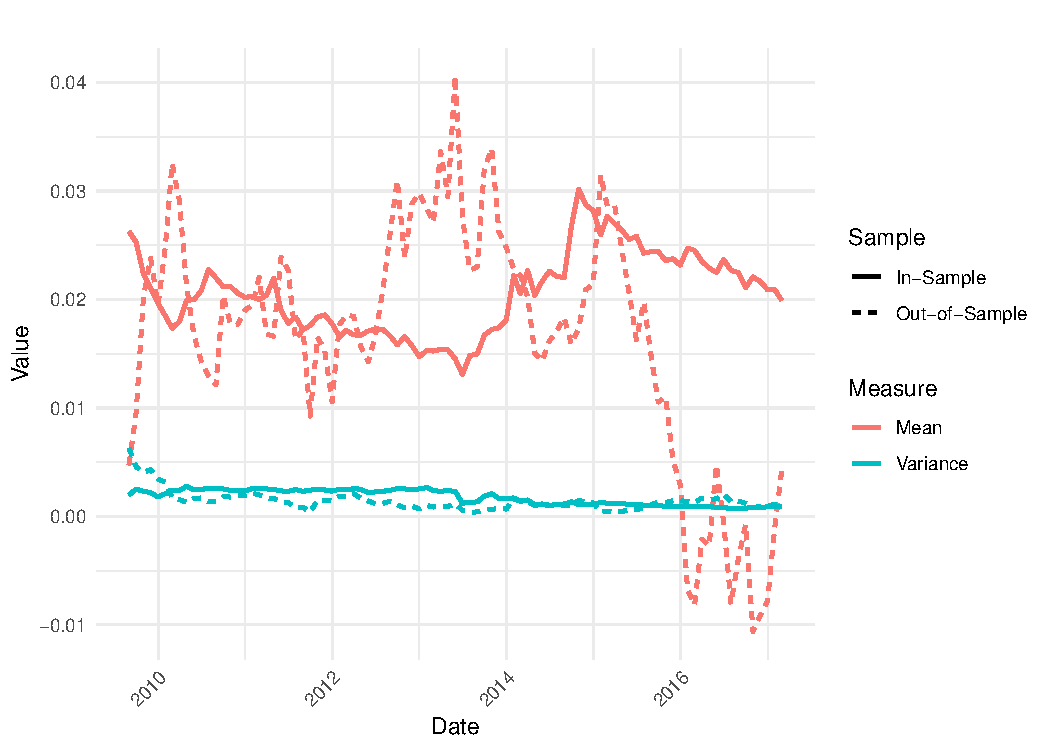
\includegraphics{NDXNES005_A1_RMD_files/figure-latex/unnamed-chunk-17-1.pdf}

\begin{Shaded}
\begin{Highlighting}[]
\NormalTok{p2}
\end{Highlighting}
\end{Shaded}

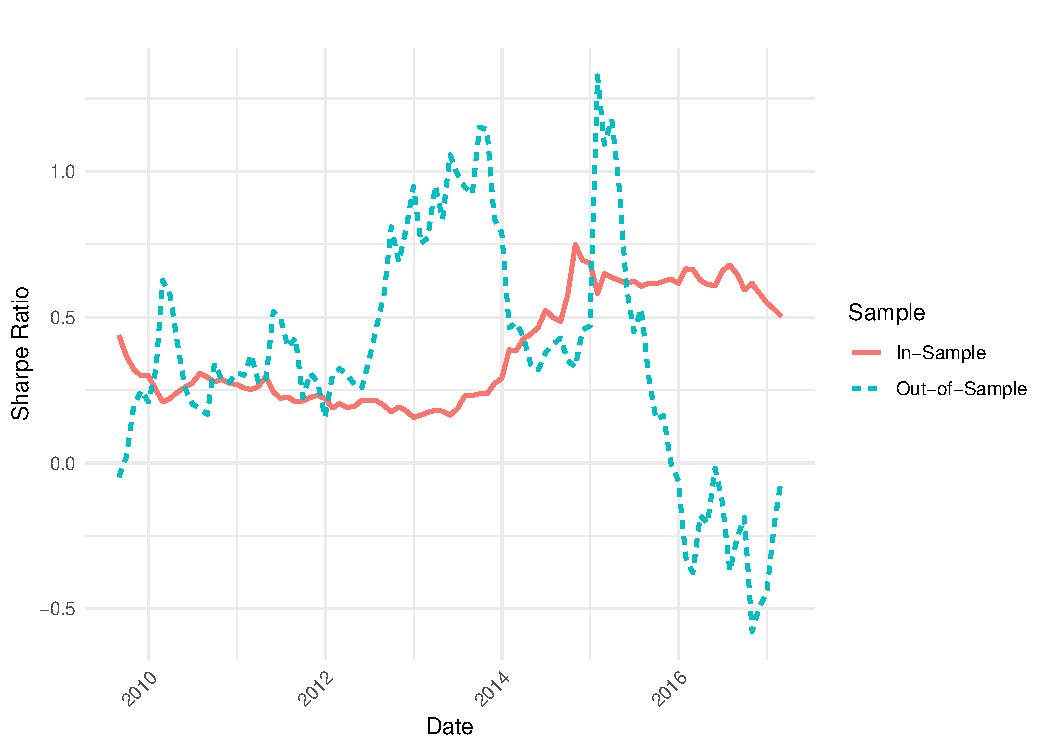
\includegraphics{NDXNES005_A1_RMD_files/figure-latex/unnamed-chunk-17-2.pdf}

\subsubsection{2.7 Buy and Hold Portfolio
Simulation}\label{buy-and-hold-portfolio-simulation}

\begin{Shaded}
\begin{Highlighting}[]
\CommentTok{\# This section calculates portfolio returns, update weights due to price changes, renormalises, and accumulate portfolio value over the test period}

\NormalTok{BH\_results }\OtherTok{\textless{}{-}} \FunctionTok{list}\NormalTok{()}

\ControlFlowTok{for}\NormalTok{(idx }\ControlFlowTok{in} \FunctionTok{seq\_along}\NormalTok{(results)) \{}
  
  \CommentTok{\# test period dates from results}
\NormalTok{  tst.period }\OtherTok{\textless{}{-}}\NormalTok{ results[[idx]]}\SpecialCharTok{$}\NormalTok{tst.period}
\NormalTok{  tst.start }\OtherTok{\textless{}{-}} \FunctionTok{as.Date}\NormalTok{(}\FunctionTok{substr}\NormalTok{(tst.period,}\DecValTok{1}\NormalTok{,}\DecValTok{10}\NormalTok{))}
\NormalTok{  tst.end   }\OtherTok{\textless{}{-}} \FunctionTok{as.Date}\NormalTok{(}\FunctionTok{substr}\NormalTok{(tst.period,}\DecValTok{14}\NormalTok{,}\DecValTok{23}\NormalTok{))}
\NormalTok{ tst.rets }\OtherTok{\textless{}{-}}\NormalTok{ rets\_opt[}\FunctionTok{as.Date}\NormalTok{(}\FunctionTok{index}\NormalTok{(rets\_opt)) }\SpecialCharTok{\textgreater{}=}\NormalTok{ tst.start }\SpecialCharTok{\&} 
                       \FunctionTok{as.Date}\NormalTok{(}\FunctionTok{index}\NormalTok{(rets\_opt)) }\SpecialCharTok{\textless{}=}\NormalTok{ tst.end, ,drop}\OtherTok{=}\ConstantTok{FALSE}\NormalTok{]}

\NormalTok{  w0 }\OtherTok{\textless{}{-}}\NormalTok{ results[[idx]]}\SpecialCharTok{$}\NormalTok{weights}
\NormalTok{  n\_assets }\OtherTok{\textless{}{-}} \FunctionTok{ncol}\NormalTok{(tst.rets)}
\NormalTok{  n\_obs }\OtherTok{\textless{}{-}} \FunctionTok{nrow}\NormalTok{(tst.rets)}
  
  \CommentTok{\# if tst.rets is empty}
  \ControlFlowTok{if}\NormalTok{(n\_obs }\SpecialCharTok{==} \DecValTok{0}\NormalTok{) }\ControlFlowTok{next}
  
\NormalTok{  Wts }\OtherTok{\textless{}{-}} \FunctionTok{matrix}\NormalTok{(}\DecValTok{0}\NormalTok{, }\AttributeTok{nrow=}\NormalTok{n\_obs, }\AttributeTok{ncol=}\NormalTok{n\_assets)}
\NormalTok{  portRet }\OtherTok{\textless{}{-}} \FunctionTok{numeric}\NormalTok{(n\_obs)}
\NormalTok{  portPrc }\OtherTok{\textless{}{-}} \FunctionTok{numeric}\NormalTok{(n\_obs)}
\NormalTok{  portPrc[}\DecValTok{1}\NormalTok{] }\OtherTok{\textless{}{-}} \DecValTok{1}
\NormalTok{  Wts[}\DecValTok{1}\NormalTok{,] }\OtherTok{\textless{}{-}}\NormalTok{ w0}
  
  \ControlFlowTok{for}\NormalTok{(t }\ControlFlowTok{in} \DecValTok{1}\SpecialCharTok{:}\NormalTok{n\_obs)\{}
\NormalTok{    portRet[t] }\OtherTok{\textless{}{-}} \FunctionTok{sum}\NormalTok{(Wts[t,] }\SpecialCharTok{*} \FunctionTok{as.numeric}\NormalTok{(tst.rets[t,]))}
\NormalTok{    portPrc[t] }\OtherTok{\textless{}{-}} \FunctionTok{ifelse}\NormalTok{(t}\SpecialCharTok{==}\DecValTok{1}\NormalTok{, }\DecValTok{1}\SpecialCharTok{*}\NormalTok{(}\DecValTok{1}\SpecialCharTok{+}\NormalTok{portRet[t]), portPrc[t}\DecValTok{{-}1}\NormalTok{]}\SpecialCharTok{*}\NormalTok{(}\DecValTok{1}\SpecialCharTok{+}\NormalTok{portRet[t]))}
    
    \ControlFlowTok{if}\NormalTok{(t }\SpecialCharTok{\textless{}}\NormalTok{ n\_obs)\{}
\NormalTok{      Wts[t}\SpecialCharTok{+}\DecValTok{1}\NormalTok{,] }\OtherTok{\textless{}{-}}\NormalTok{ Wts[t,] }\SpecialCharTok{*}\NormalTok{ (}\DecValTok{1} \SpecialCharTok{+} \FunctionTok{as.numeric}\NormalTok{(tst.rets[t,]))}
\NormalTok{      Wts[t}\SpecialCharTok{+}\DecValTok{1}\NormalTok{,] }\OtherTok{\textless{}{-}}\NormalTok{ Wts[t}\SpecialCharTok{+}\DecValTok{1}\NormalTok{,] }\SpecialCharTok{/} \FunctionTok{sum}\NormalTok{(Wts[t}\SpecialCharTok{+}\DecValTok{1}\NormalTok{,])}
\NormalTok{    \}}
\NormalTok{  \}}
  
\NormalTok{  BH\_results[[idx]] }\OtherTok{\textless{}{-}} \FunctionTok{list}\NormalTok{(}
    \AttributeTok{weights=}\NormalTok{Wts,}
    \AttributeTok{asset\_names=}\FunctionTok{colnames}\NormalTok{(tst.rets),}
    \AttributeTok{portPrc=}\NormalTok{portPrc,}
    \AttributeTok{portRet=}\NormalTok{portRet,}
    \AttributeTok{dates=}\FunctionTok{index}\NormalTok{(tst.rets)}
\NormalTok{  )}
\NormalTok{\}}
\end{Highlighting}
\end{Shaded}

\subsubsection{2.8 Final cumulative
return}\label{final-cumulative-return-1}

\begin{Shaded}
\begin{Highlighting}[]
\NormalTok{plot\_df }\OtherTok{\textless{}{-}} \FunctionTok{pivot\_longer}\NormalTok{(BH\_summary, }\AttributeTok{cols =} \FunctionTok{c}\NormalTok{(BH\_Return, Tangency\_Expected),}\AttributeTok{names\_to =} \StringTok{"Strategy"}\NormalTok{, }\AttributeTok{values\_to =} \StringTok{"Value"}\NormalTok{)}

\FunctionTok{ggplot}\NormalTok{(plot\_df, }\FunctionTok{aes}\NormalTok{(}\AttributeTok{x =}\NormalTok{ Window, }\AttributeTok{y =}\NormalTok{ Value, }\AttributeTok{color =}\NormalTok{ Strategy)) }\SpecialCharTok{+}
  \FunctionTok{geom\_line}\NormalTok{(}\AttributeTok{linewidth =} \FloatTok{0.9}\NormalTok{) }\SpecialCharTok{+}
  \FunctionTok{geom\_point}\NormalTok{(}\AttributeTok{size =} \FloatTok{1.5}\NormalTok{) }\SpecialCharTok{+}
  \FunctionTok{labs}\NormalTok{(}
    \AttributeTok{title =} \StringTok{""}\NormalTok{,}
    \AttributeTok{x =} \StringTok{"Test Window"}\NormalTok{, }\AttributeTok{y =} \StringTok{"Cumulative Return"}\NormalTok{,}
    \AttributeTok{color =} \StringTok{"Portfolio Strategy"}
\NormalTok{  ) }\SpecialCharTok{+}
  \FunctionTok{scale\_color\_manual}\NormalTok{(}
    \AttributeTok{values =} \FunctionTok{c}\NormalTok{(}\StringTok{"BH\_Return"} \OtherTok{=} \StringTok{"red"}\NormalTok{, }\StringTok{"Tangency\_Expected"} \OtherTok{=} \StringTok{"blue"}\NormalTok{),}
    \AttributeTok{labels =} \FunctionTok{c}\NormalTok{(}\StringTok{"BH\_Return"} \OtherTok{=} \StringTok{"Buy{-}and{-}Hold"}\NormalTok{, }\StringTok{"Tangency\_Expected"} \OtherTok{=} \StringTok{"Tangency Portfolio Expected"}\NormalTok{)}
\NormalTok{  ) }\SpecialCharTok{+}
  \FunctionTok{theme\_minimal}\NormalTok{() }\SpecialCharTok{+}
  \FunctionTok{theme}\NormalTok{(}\AttributeTok{axis.text.x =} \FunctionTok{element\_text}\NormalTok{(}\AttributeTok{angle =} \DecValTok{0}\NormalTok{, }\AttributeTok{hjust =} \FloatTok{0.5}\NormalTok{))}
\end{Highlighting}
\end{Shaded}

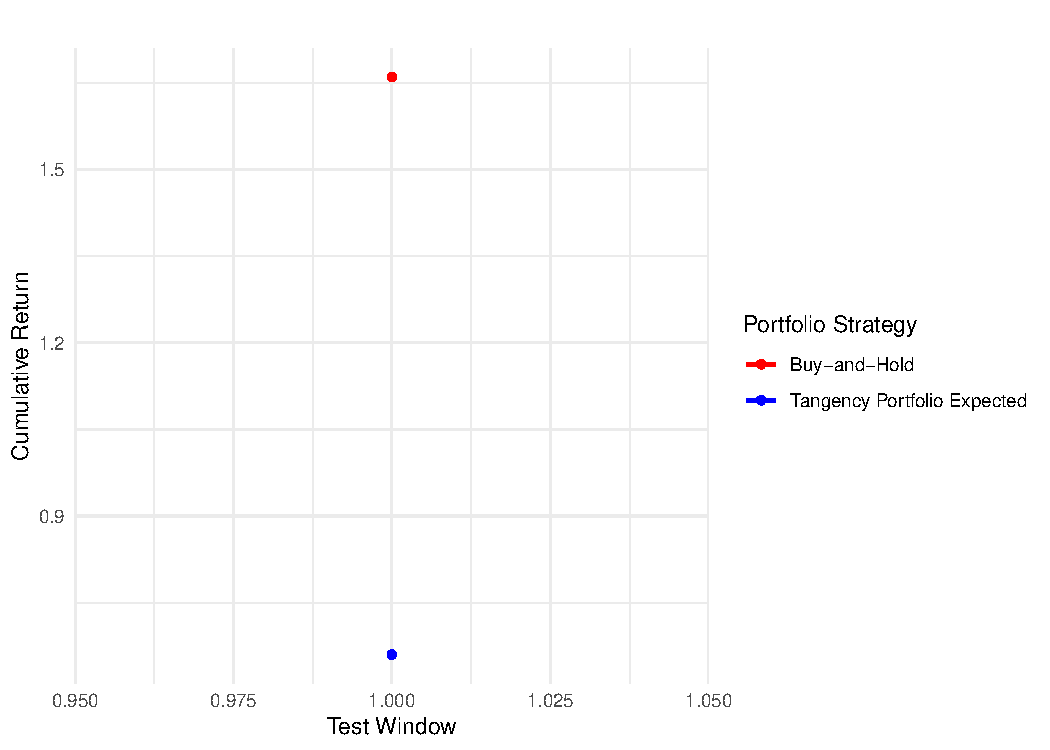
\includegraphics{NDXNES005_A1_RMD_files/figure-latex/unnamed-chunk-19-1.pdf}

\subsubsection{2.9 Tangency Portfolio Weights using
heatmap}\label{tangency-portfolio-weights-using-heatmap}

\begin{Shaded}
\begin{Highlighting}[]
\NormalTok{weights\_df }\OtherTok{\textless{}{-}} \FunctionTok{do.call}\NormalTok{(rbind, }\FunctionTok{lapply}\NormalTok{(}\FunctionTok{seq\_along}\NormalTok{(results), }\ControlFlowTok{function}\NormalTok{(i) \{}
\NormalTok{  n\_assets }\OtherTok{\textless{}{-}} \FunctionTok{length}\NormalTok{(results[[i]]}\SpecialCharTok{$}\NormalTok{weights)}
  \FunctionTok{data.frame}\NormalTok{(}
    \AttributeTok{Window =}\NormalTok{ i, }\CommentTok{\# numeric window index}
    \AttributeTok{Asset  =}\NormalTok{ results[[i]]}\SpecialCharTok{$}\NormalTok{assets, }\CommentTok{\#asset names}
    \AttributeTok{Weight =}\NormalTok{ results[[i]]}\SpecialCharTok{$}\NormalTok{weights,}\CommentTok{\#corresponding weights}
    \AttributeTok{stringsAsFactors =} \ConstantTok{FALSE}
\NormalTok{  )}
\NormalTok{\}))}

 \CommentTok{\# Tangency Portfolio Weights Evolution}
\FunctionTok{ggplot}\NormalTok{(weights\_df, }\FunctionTok{aes}\NormalTok{(}\AttributeTok{x=}\NormalTok{Window, }\AttributeTok{y=}\NormalTok{Asset, }\AttributeTok{fill=}\NormalTok{Weight)) }\SpecialCharTok{+}
  \FunctionTok{geom\_tile}\NormalTok{(}\AttributeTok{color=}\StringTok{"white"}\NormalTok{) }\SpecialCharTok{+}
  \FunctionTok{scale\_fill\_gradient}\NormalTok{(}\AttributeTok{low=}\StringTok{"white"}\NormalTok{, }\AttributeTok{high=}\StringTok{"steelblue"}\NormalTok{) }\SpecialCharTok{+}
  \FunctionTok{scale\_x\_continuous}\NormalTok{(}
    \AttributeTok{breaks =} \FunctionTok{seq}\NormalTok{(}\FunctionTok{min}\NormalTok{(weights\_df}\SpecialCharTok{$}\NormalTok{Window), }\FunctionTok{max}\NormalTok{(weights\_df}\SpecialCharTok{$}\NormalTok{Window), }\AttributeTok{by=}\DecValTok{5}\NormalTok{) }
\NormalTok{  ) }\SpecialCharTok{+}
  \FunctionTok{labs}\NormalTok{(}
    \AttributeTok{title=}\StringTok{""}\NormalTok{,}
    \AttributeTok{x=}\StringTok{"Training Window"}\NormalTok{, }\AttributeTok{y=}\StringTok{"Asset"}\NormalTok{, }\AttributeTok{fill=}\StringTok{"Weight"}
\NormalTok{  ) }\SpecialCharTok{+}
  \FunctionTok{theme\_minimal}\NormalTok{() }\SpecialCharTok{+}
  \FunctionTok{theme}\NormalTok{(}\AttributeTok{axis.text.x =} \FunctionTok{element\_text}\NormalTok{(}\AttributeTok{angle=}\DecValTok{45}\NormalTok{, }\AttributeTok{hjust=}\DecValTok{1}\NormalTok{))}
\end{Highlighting}
\end{Shaded}

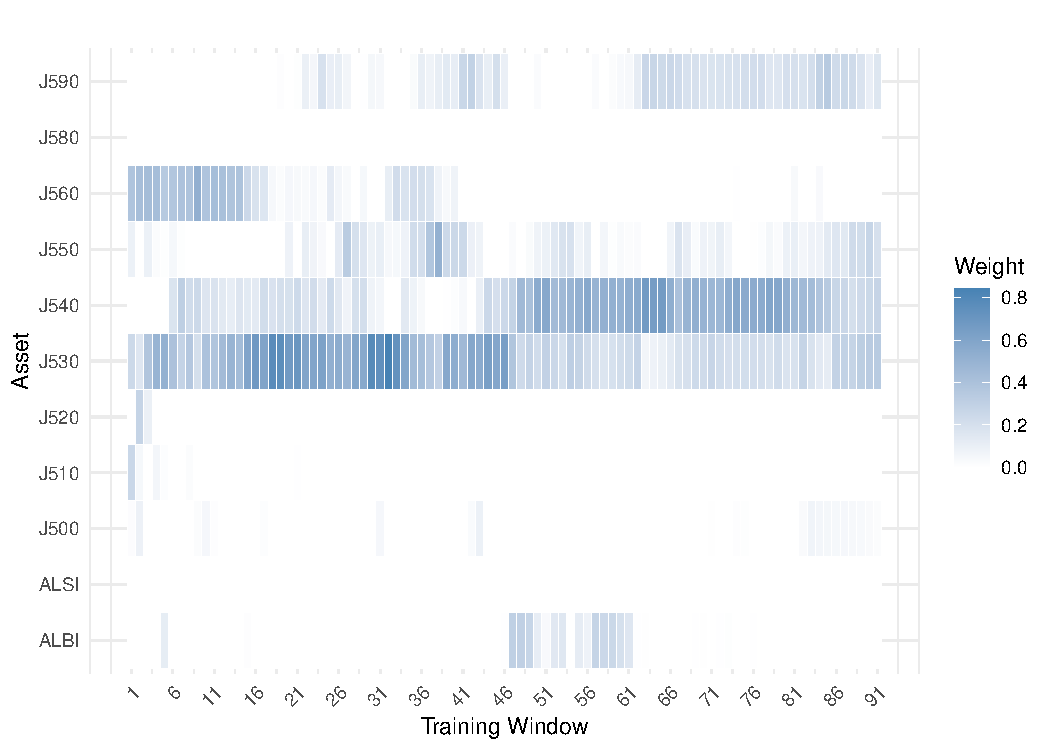
\includegraphics{NDXNES005_A1_RMD_files/figure-latex/unnamed-chunk-20-1.pdf}

\subsubsection{2.10 Cumulative Out-of-Sample Performance vs Buy
Hold}\label{cumulative-out-of-sample-performance-vs-buy-hold}

\begin{Shaded}
\begin{Highlighting}[]
\CommentTok{\#out{-}of{-}sample returns }
\NormalTok{OOS\_ret }\OtherTok{\textless{}{-}} \FunctionTok{sapply}\NormalTok{(results, }\ControlFlowTok{function}\NormalTok{(x) \{}
\NormalTok{  val }\OtherTok{\textless{}{-}}\NormalTok{ x}\SpecialCharTok{$}\NormalTok{mu\_OOS}
  \ControlFlowTok{if}\NormalTok{(}\FunctionTok{is.null}\NormalTok{(val) }\SpecialCharTok{||} \SpecialCharTok{!}\FunctionTok{is.finite}\NormalTok{(val)) }\FunctionTok{return}\NormalTok{(}\ConstantTok{NA}\NormalTok{)}
  \FunctionTok{as.numeric}\NormalTok{(val)}
\NormalTok{\})}
\CommentTok{\#remove NAs}
\NormalTok{OOS\_ret }\OtherTok{\textless{}{-}}\NormalTok{ OOS\_ret[}\SpecialCharTok{!}\FunctionTok{is.na}\NormalTok{(OOS\_ret)]}
\NormalTok{OOS\_ret }\OtherTok{\textless{}{-}} \FunctionTok{as.numeric}\NormalTok{(OOS\_ret) }
\CommentTok{\#Calculate cumulative wealth}
\NormalTok{cum\_OOS }\OtherTok{\textless{}{-}} \FunctionTok{cumprod}\NormalTok{(}\DecValTok{1} \SpecialCharTok{+}\NormalTok{ OOS\_ret)}
\CommentTok{\#  Buy{-}and{-}Hold}
\NormalTok{BH\_ret }\OtherTok{\textless{}{-}} \FunctionTok{sapply}\NormalTok{(BH\_results, }\ControlFlowTok{function}\NormalTok{(x) \{}
  \ControlFlowTok{if}\NormalTok{(}\FunctionTok{is.null}\NormalTok{(x}\SpecialCharTok{$}\NormalTok{portRet)) }\FunctionTok{return}\NormalTok{(}\ConstantTok{NA}\NormalTok{)}
  \FunctionTok{mean}\NormalTok{(}\FunctionTok{as.numeric}\NormalTok{(x}\SpecialCharTok{$}\NormalTok{portRet), }\AttributeTok{na.rm=}\ConstantTok{TRUE}\NormalTok{)}
\NormalTok{\})}
\NormalTok{BH\_ret }\OtherTok{\textless{}{-}}\NormalTok{ BH\_ret[}\SpecialCharTok{!}\FunctionTok{is.na}\NormalTok{(BH\_ret)]}
\NormalTok{BH\_ret }\OtherTok{\textless{}{-}} \FunctionTok{as.numeric}\NormalTok{(BH\_ret)}
\NormalTok{cum\_BH }\OtherTok{\textless{}{-}} \FunctionTok{cumprod}\NormalTok{(}\DecValTok{1} \SpecialCharTok{+}\NormalTok{ BH\_ret)}

\DocumentationTok{\#\# keeps results with valid numeric data}
\NormalTok{val.res }\OtherTok{\textless{}{-}}\NormalTok{ results[}\FunctionTok{sapply}\NormalTok{(results, }\ControlFlowTok{function}\NormalTok{(x) }\SpecialCharTok{!}\FunctionTok{is.null}\NormalTok{(x}\SpecialCharTok{$}\NormalTok{mu\_OOS) }\SpecialCharTok{\&\&} \FunctionTok{is.finite}\NormalTok{(x}\SpecialCharTok{$}\NormalTok{mu\_OOS))]}

\CommentTok{\#end{-}of{-}test{-}period dates as character}
\NormalTok{p.dates\_char }\OtherTok{\textless{}{-}} \FunctionTok{sapply}\NormalTok{(val.res, }\ControlFlowTok{function}\NormalTok{(x) \{}
  \FunctionTok{tail}\NormalTok{(}\FunctionTok{strsplit}\NormalTok{(x}\SpecialCharTok{$}\NormalTok{tst.period, }\StringTok{" / "}\NormalTok{)[[}\DecValTok{1}\NormalTok{]], }\DecValTok{1}\NormalTok{)}
\NormalTok{\})}

\NormalTok{p.dates }\OtherTok{\textless{}{-}} \FunctionTok{as.Date}\NormalTok{(}\FunctionTok{unlist}\NormalTok{(p.dates\_char), }\AttributeTok{format=}\StringTok{"\%Y{-}\%m{-}\%d"}\NormalTok{) }
\NormalTok{plot\_df }\OtherTok{\textless{}{-}} \FunctionTok{data.frame}\NormalTok{(}
  \AttributeTok{Date     =}\NormalTok{ p.dates,}
  \AttributeTok{Tangency =}\NormalTok{ cum\_OOS,}
  \AttributeTok{BuyHold  =}\NormalTok{ cum\_BH[}\DecValTok{1}\SpecialCharTok{:}\FunctionTok{length}\NormalTok{(cum\_OOS)]}
\NormalTok{)}

\NormalTok{df.long }\OtherTok{\textless{}{-}} \FunctionTok{pivot\_longer}\NormalTok{(plot\_df, }\AttributeTok{cols=}\FunctionTok{c}\NormalTok{(}\StringTok{"Tangency"}\NormalTok{,}\StringTok{"BuyHold"}\NormalTok{),}
                             \AttributeTok{names\_to=}\StringTok{"Strategy"}\NormalTok{, }\AttributeTok{values\_to=}\StringTok{"Cumulative\_Wealth"}\NormalTok{)}

\CommentTok{\# Cumulative Out{-}of{-}Sample Performance}
\FunctionTok{ggplot}\NormalTok{(df.long, }\FunctionTok{aes}\NormalTok{(}\AttributeTok{x=}\NormalTok{Date, }\AttributeTok{y=}\NormalTok{Cumulative\_Wealth, }\AttributeTok{color=}\NormalTok{Strategy)) }\SpecialCharTok{+}
  \FunctionTok{geom\_line}\NormalTok{(}\AttributeTok{linewidth=}\FloatTok{0.8}\NormalTok{) }\SpecialCharTok{+}
  \FunctionTok{labs}\NormalTok{(}\AttributeTok{title=}\StringTok{""}\NormalTok{,}
       \AttributeTok{x=}\StringTok{"Date"}\NormalTok{, }\AttributeTok{y=}\StringTok{"Cumulative Wealth"}\NormalTok{, }\AttributeTok{color=}\StringTok{"Strategy"}\NormalTok{) }\SpecialCharTok{+}
  \FunctionTok{scale\_color\_manual}\NormalTok{(}\AttributeTok{values=}\FunctionTok{c}\NormalTok{(}\StringTok{"blue"}\NormalTok{,}\StringTok{"red"}\NormalTok{)) }\SpecialCharTok{+}
  \FunctionTok{theme\_minimal}\NormalTok{()}
\end{Highlighting}
\end{Shaded}

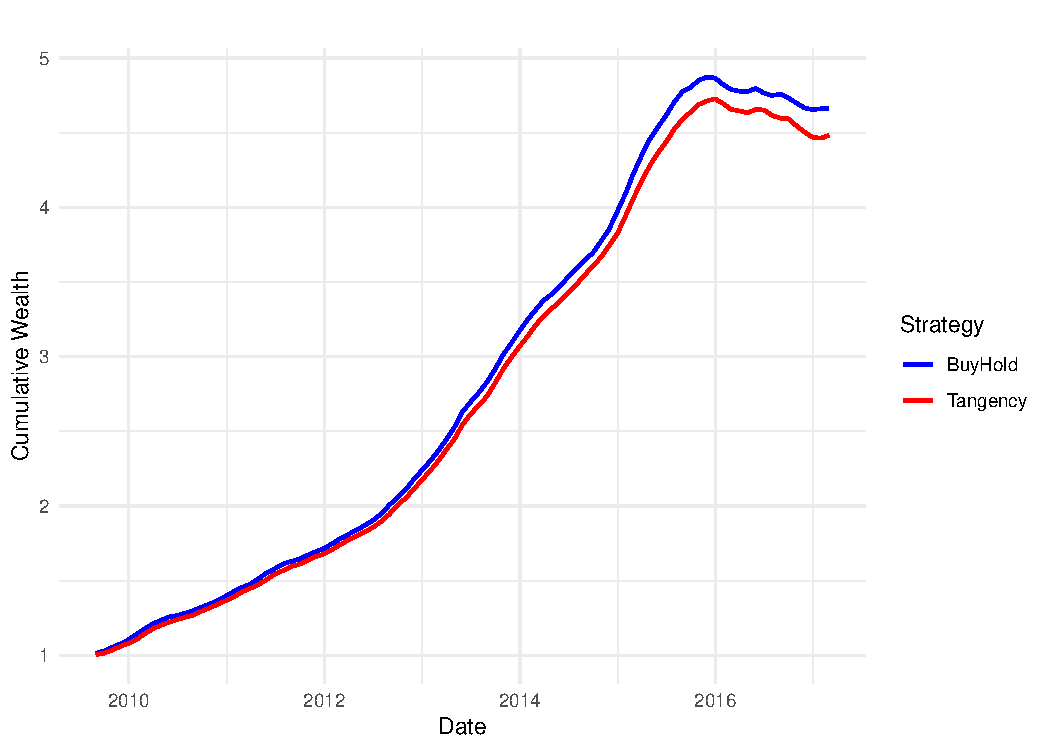
\includegraphics{NDXNES005_A1_RMD_files/figure-latex/unnamed-chunk-21-1.pdf}

\newpage

\section*{References}\label{references}
\addcontentsline{toc}{section}{References}

\phantomsection\label{refs}
\begin{CSLReferences}{1}{0}
\bibitem[\citeproctext]{ref-bailey_2014}
Bailey, D. H., \& López de Prado, M. (2014). The deflated sharpe
ratio:correcting for selection bias, BacktestOverfitting, and
non-normality. \emph{The Journal of Portfolio Management}, \emph{40},
94--107. \url{https://doi.org/10.3905/jpm.2014.40.5.094}

\bibitem[\citeproctext]{ref-bailey_2016}
Bailey, D., Borwein, J., López de Prado, M., \& Zhu, Q. J. (2016). The
probability of backtest overfitting. \emph{The Journal of Computational
Finance}. \url{https://doi.org/10.21314/jcf.2016.322}

\bibitem[\citeproctext]{ref-embrechts_1997}
Embrechts, P., Klüppelberg, C., \& Mikosch, T. (1997). \emph{Modelling
extremal events for insurance and finance}. Springer.

\bibitem[\citeproctext]{ref-fisher1928}
Fisher, R. A., \& Tippett, L. H. C. (1928). \emph{Limiting forms of the
frequency distribution of the largest or smallest member of a sample}
(Vol. 24, pp. 180--190). Cambridge University Press.

\bibitem[\citeproctext]{ref-Tim_BT}
Gebbie, T. (2025a). \emph{PortfolioTheory-backtest-001.r}. Unpublished
teaching material.

\bibitem[\citeproctext]{ref-Tim_prepmlx}
Gebbie, T. (2025b). \emph{PortfolioTheoryLecture001.mlx}. Unpublished
teaching material.

\bibitem[\citeproctext]{ref-Tim_BTmlx}
Gebbie, T. (2025c). \emph{PortfolioTheoryLecture003.pdf}. Unpublished
teaching material.

\bibitem[\citeproctext]{ref-Tim_prep}
Gebbie, T. (2025d). \emph{PortfolioTheory-PrepareData-000.r}.
Unpublished teaching material.

\bibitem[\citeproctext]{ref-gnedenko2006}
Gnedenko, B. (2006). \emph{On limit theorems for a random number of
random variables} (pp. 167--176). Springer.

\bibitem[\citeproctext]{ref-lee_2000}
Lee, W. (2000). \emph{Theory and methodology of tactical asset
allocation}. John Wiley \& Sons.

\bibitem[\citeproctext]{ref-liu_2012}
Liu, Y., Rekkas, M., \& Wong, A. (2012). Inference for the sharpe ratio
using a likelihood-based approach. \emph{Journal of Probability and
Statistics}, \emph{2012}, 1--24.
\url{https://doi.org/10.1155/2012/878561}

\bibitem[\citeproctext]{ref-lo_2002}
Lo, A. W. (2002). The statistics of sharpe ratios. \emph{Financial
Analysts Journal}, \emph{58}, 36--52.
\url{https://doi.org/10.2469/faj.v58.n4.2453}

\bibitem[\citeproctext]{ref-resnick_2008}
Resnick, S. I. (2008). \emph{Extreme values, regular variation and point
processes}. Springer, Cop.

\end{CSLReferences}

\end{document}
